%%%%(c)
%%%%(c)  This file is a portion of the source for the textbook
%%%%(c)
%%%%(c)    Abstract Algebra: Theory and Applications
%%%%(c)    Copyright 1997 by Thomas W. Judson
%%%%(c)
%%%%(c)  See the file COPYING.txt for copying conditions
%%%%(c)
%%%%(c)
\documentclass[11pt]{book}

\usepackage{enumerate} %% CPT

\usepackage{graphicx}
\usepackage{amssymb}
\usepackage{epstopdf}
\usepackage{amsmath}
\usepackage{amscd}   %% redundant after tikz conversions?
\usepackage{multicol}
\usepackage{longtable}
\usepackage{makeidx}
\usepackage{placeins}%  CPT
\usepackage{url}

\usepackage{tikz}
\newcommand{\tikzpreface}[1]{\relax}

\usepackage{float}
\restylefloat{table}

\usepackage{hyperref}
\hypersetup{
  colorlinks   = true, %Colours links instead of ugly boxes
  urlcolor     = blue, %Colour for external hyperlinks
  linkcolor    = blue, %Colour of internal links
  citecolor   = red %Colour of citations
}

% Widows and orphans, from VCU edition
% R Beezer, 2010/06/14
\widowpenalty=10000
\clubpenalty=10000
\raggedbottom

\setlength{\fboxrule}{0.5pt}

\setlength{\parskip}{1ex plus 0.5ex minus 0.2ex} % Added to put spaces between paragraphs.

%%%%(c)
%%%%(c)  This file is a portion of the source for the textbook
%%%%(c)
%%%%(c)    Abstract Algebra: Theory and Applications
%%%%(c)    Copyright 1997 by Thomas W. Judson
%%%%(c)
%%%%(c)  See the file COPYING.txt for copying conditions
%%%%(c)
%%%%(c)
%%%%%%%%%%%%%%%%%%%%%%%%%%%%%%%%%%%%%%%%%%%%%%%%%%
%
%  Macros for algebra text
%
%%%%%%%%%%%%%%%%%%%%%%%%%%%%%%%%%%%%%%%%%%%%%%%%%%


%********theorems, propositions, lemmas, corollaries, proofs**

%% RAB, 2008/01/28
%%   Ditched [chapter] at end of three subsidiary environments
%%   The "[chapter]" was being printed

\newtheorem{theorem}{Theorem}[chapter]
  
\newtheorem{proposition}[theorem]{Proposition}
 
\newtheorem{lemma}[theorem]{Lemma}
 
\newtheorem{corollary}[theorem]{Corollary}
 
\newenvironment{proof}{\noindent {\sc
Proof.}}{\hspace{\fill} $\square$}


%********New commands******

\newcommand{\notdivide}{{\not{\mid}}} %Changed command from \notmid to avoid conflict with tikz - TWJ 5/6/2010

\newcommand{\notsubset}{\not\subset}

\newcommand{\lcm}{\operatorname{lcm}}

\newcommand{\Hom}{\operatorname{Hom}} %Added operator \Hom - TWJ 8/19/2010

\newcommand{\cis}{\operatorname{cis}}

\newcommand{\exrule}{\vspace{-0.3in} \noindent \rule{5.00in}{.5pt}}
		%********rule for exercise headings*******

\newcommand{\drawbox}{\raisebox{3pt}{\framebox[1.7in]{\hspace*{1in}}}}
		%********draws an empty box**********

\newcommand{\histbox}{\raisebox{3pt}{\hspace*{4pt}\framebox[.5in]{\hspace*{.25in}}}}
		%********draws an empty box**********


%********New fonts*************

\newfont{\bfi}{cmbxti10 scaled\magstephalf}  	%11pt bold italic

\newfont{\cmss}{cmss10}				%10pt sans serif

\newfont{\histf}{cmr10}				%10pt roman
						%Historical notes








%********Headings for historical notes*****


\newcommand{\histhead}{
\vspace{3ex} \noindent \drawbox \hfill \hspace*{4pt}
{\bfi Historical Note} \hfill \drawbox
\vspace{2ex}
}


%%%%%%%%%%%%%%%%%%%%%%%%%%%%%%%%%%%%%
%
%  ETP Modifications:
%	- Chapters start new left or right, not new right
%	- Float numbers are to be bold and punctuated with a period, not colon
%	- Allow larger floats on a text page
%	- Re-work the Chapter Opener
%
%%%%%%%%%%%%%%%%%%%%%%%%%%%%%%%%%%%%%


\makeatletter

\setcounter{topnumber}{2}	% Default parameter value from LaTeX book style
\def\topfraction{.7}		% Default parameter value from LaTeX book style
\setcounter{bottomnumber}{1}	% Default parameter value from LaTeX book style
\def\bottomfraction{.3}		% Default parameter value from LaTeX book style
\setcounter{totalnumber}{3}	% Default parameter value from LaTeX book style
\def\textfraction{.15}		% CHANGE: parameter was {.2}
\def\floatpagefraction{.7}	% CHANGE: parameter was {.5}




% Modified to remove the period after the chapter and section numbers
% in the running heads
\def\ps@headings{\let\@mkboth\markboth
\def\@oddfoot{}\def\@evenfoot{}\def\@evenhead{\rm \thepage\hfil \sl
\leftmark}\def\@oddhead{\hbox{}\sl \rightmark \hfil
\rm\thepage}\def\chaptermark##1{\markboth {\uppercase{\ifnum \c@secnumdepth
>\m@ne
 \@chapapp\ \thechapter \ \ \ \fi ##1}}{}}\def\sectionmark##1{\markright
{\uppercase{\ifnum \c@secnumdepth >\z@
 \thesection \ \ \ \fi ##1}}}}
\def\ps@myheadings{\let\@mkboth\@gobbletwo
\def\@oddhead{\hbox{}\sl\rightmark \hfil
\rm\thepage}\def\@oddfoot{}\def\@evenhead{\rm \thepage\hfil\sl\leftmark\hbox
{}}\def\@evenfoot{}\def\chaptermark##1{}\def\sectionmark##1{}%
\def\subsectionmark##1{}}



% Modified to embolden the figure (or table) number and punctuate with period
\long\def\@makecaption#1#2{
 \vskip 10pt
 \setbox\@tempboxa\hbox{{\bf #1.} #2}
 \ifdim \wd\@tempboxa >\hsize{\bf #1.} #2\par \else \hbox
to\hsize{\hfil\box\@tempboxa\hfil}
 \fi}


% RAB, 2010/06/17
% Fancy chapter headings for print versions
% Do nothing for tex4ht versions
\font\bigbolditalic=cmsl10 scaled\magstep5
\def\@makechapterhead#1{%\vspace*{50pt}
 { \parindent 0pt \centering% was\raggedright
 \ifnum \c@secnumdepth >\m@ne\rule{2in}{.5pt}\hfill\raisebox{-.1in}{\fbox{\fbox{\bigbolditalic\thechapter\/}}}\hfill\rule{2in}{.5pt}\par%

 \vskip 20pt \fi \Huge \bf #1\par%
 \nobreak \vskip 40pt \framebox[\hsize]{\hspace*{1in}}}%
 \vskip 36pt plus 12pt minus 6pt }%
%
\def\@makeschapterhead#1{%\vspace*{50pt}
 { \parindent 0pt \centering% was \raggedright
 \hrule height .5pt\vspace{40pt}%
 \huge \bf #1\par%
 \nobreak \vskip 40pt \framebox[\hsize]{\hspace*{1in}}}%
 \vskip 36pt plus 12pt minus 6pt }%
%
% \clearpage below was \cleardoublepage
\def\chapter{\clearpage \thispagestyle{plain} \global\@topnum\z@%
\@afterindentfalse \secdef\@chapter\@schapter}





\makeatother





% Per-chapter items
\newcommand{\chaplabel}{\relax}
\newcounter{example}[chapter]

% Usage: \chap{title}{label}
\newcommand{\chap}[2]{
     \setcounter{example}{0}%
     \renewcommand{\chaplabel}{#2}
     \chapter{#1}\label{#2}
}

% Examples as environment
\newenvironment{example}[1]
  {\refstepcounter{example}{\bigskip\noindent\bf Example~\arabic{example}.}\label{example:\chaplabel:#1}}
  {\hspace\fill$\blacklozenge$\par\medskip}

%%% Other environments (CPT, Dec 22 2010) %%%
\newenvironment{prop}[1]
  {\refstepcounter{example}{\bigskip\noindent\bf Proposition~\arabic{example}.}\label{proposition:\chaplabel:#1}}
  {\par\medskip}

\newenvironment{exercise}[1]
  {\refstepcounter{example}{\bigskip\noindent\bf Exercise~\arabic{example}.}\label{exercise:\chaplabel:#1}}
  {\hspace\fill$\lozenge$\par\medskip}

\newenvironment{defn}
  {\refstepcounter{example}{\bigskip\noindent\bf Definition~\arabic{example}.}}
  {\hspace\fill$\triangle$\par\medskip}

\newenvironment{rem}
  {\refstepcounter{example}{\bigskip\noindent\bf Remark~\arabic{example}.}}
  {\hspace\fill$\triangle$\par\medskip}

\newenvironment{notation}[1]
  {\refstepcounter{example}{\bigskip\noindent\bf Notation~\arabic{example}.}\label{notation:\chaplabel:#1}}
  {\hspace\fill$\triangle$\par\medskip}

%%% Legacy from P&C
\newenvironment{thm}
  {\refstepcounter{example}{\bigskip\noindent\bf Proposition~\arabic{example}.}}
  {\par\medskip}

\newenvironment{eg}
  {\refstepcounter{example}{\bigskip\noindent\bf Example~\arabic{example}.}}
  {\hspace\fill$\lozenge$\par\medskip}

\newenvironment{exer}
  {\refstepcounter{example}{\bigskip\noindent\bf Exercise~\arabic{example}.}}
  {\hspace\fill$\lozenge$\par\medskip}

\newenvironment{exers}
  {\bigskip {\bf Exercises} \medskip}
  {\hspace\fill$\lozenge$\par\medskip}

\newenvironment{summary}
  {\bigskip {\bf Summary} \medskip \begin{itemize}}
  {\end{itemize}\hspace\fill$\lozenge$\par\medskip}

\newenvironment{problist}
  {\bigskip {\bf Problem List} \medskip \begin{itemize}}
  {\end{itemize}\hspace\fill$\lozenge$\par\medskip}

\newenvironment{scratchwork}
  {\medskip \par}
  {\medskip \par}

\newenvironment{solution}
  {\bigskip {\bf Solution} \medskip}
  {\hspace\fill$\lozenge$\par\medskip}

\newenvironment{warn}
  {\bigskip \noindent{\bf Warning} \medskip}
  {\hspace\fill$\lozenge$\par\medskip}

{\newcommand{\chapterletter}[1]{#1}}

\renewenvironment{corollary}
  {\refstepcounter{example}{\bigskip\noindent\bf Corollary~\arabic{example}.}}
  {\par\medskip}


% New commands defined by CPT (legacy from P & C)
\newcommand{\var}[1]{\sf{#1}} 
\newcommand{\bfii}[1]{\textbf{\textit{{#1}}}}
\newcommand{\terminology}[1]{\bfii{ #1}} 
\newcommand{\hint}[1]{\emph{#1}} 
\newcommand{\cref}[1]{\sf{\bfii{ #1}}} %%%% Cross-reference, legacy from P & C
\newcommand{\Cref}[1]{\sf{\bfii{ #1}}} %%%% Cross-reference, legacy from P & C
\newcommand{\real}{\mathbb{R}}
\newcommand{\rational}{\mathbb{Q}}
\newcommand{\integer}{\mathbb{Z}}
\newcommand{\univ}{\mathbb{U}}
\newcommand{\factoidbox}[1]{#1}
\newcommand{\eif}{\Rightarrow}
\newcommand{\eiff}{\Leftrightarrow}
\newcommand{\qedhere}{\Box}
\newcommand{\qed}{\Box}
\newcommand{\compose}{\circ}
\newcommand{\bigset}[1]{ \left\{ #1 \right\}}
\newcommand{\Id}{\sf{Id}}
\newcommand{\rel}{\sim}




\renewcommand{\ref}{\href}


%
\makeindex
%
\pagestyle{headings}

% Following is recommended from http://mintaka.sdsu.edu/GF/bibliog/latex/floats.html
% Alter some LaTeX defaults for better treatment of figures:
    % See p.105 of "TeX Unbound" for suggested values.
    % See pp. 199-200 of Lamport's "LaTeX" book for details.
    %   General parameters, for ALL pages:
    \renewcommand{\topfraction}{0.9}	% max fraction of floats at top
    \renewcommand{\bottomfraction}{0.8}	% max fraction of floats at bottom
    %   Parameters for TEXT pages (not float pages):
    \setcounter{topnumber}{2}
    \setcounter{bottomnumber}{2}
    \setcounter{totalnumber}{4}     % 2 may work better
    \setcounter{dbltopnumber}{2}    % for 2-column pages
   \renewcommand{\dbltopfraction}{0.9}	% fit big float above 2-col. text
    \renewcommand{\textfraction}{0.07}	% allow minimal text w. figs
    %   Parameters for FLOAT pages (not text pages):
    \renewcommand{\floatpagefraction}{0.7}	% require fuller float pages
	% N.B.: floatpagefraction MUST be less than topfraction !!
    \renewcommand{\dblfloatpagefraction}{0.7}	% require fuller float pages

	% remember to use [htp] or [htpb] for placement

\begin{document}
%
\begin{titlepage}
\title{Elementary Abstract Algebra: Examples and Applications}
\author{Justin Hill, Chris Thron}
\begin{center}
\vspace{3.5cm}
{\huge \textbf{ Elementary Abstract Algebra: Examples and Applications}}\\[1cm]
Conceived by \\ [0.5 cm]
{ \textbf{Justin Hill, Chris Thron (\emph{editor})} } \\
Texas A\&M University -- Central Texas \\[0.4cm]
Incorporating source materials by\\[0.4cm]
\textbf{Thomas Judson} (Stephen F. Austin State University) \\
\textbf{Dave Witte  Morris and Joy Morris} (University of Lethbridge) \\[0.4cm]
Additional contributions by\\[0.4cm]
\textbf {Johnny Watts, David Weathers} (A\&M -- Central Texas)\\[0.4cm]

\vfill

% Bottom of the page
{\large \today}\\ [1 cm]
This book is offered under the Creative Commons license (Attribution-NonCommercial-ShareAlike 2.0).

\end{center}
\end{titlepage}
\vspace{4cm}

\noindent
Material from "Abstract Algebra, Theory and Applications" by Thomas Judson may be found throughout much of the  book. 
A current version of "Abstract Algebra, Theory and Applications" may be found at \url{abstract.ups.edu}.\\[0.5cm]
Chapters 4 and 5 are largely based on "Proofs and Concepts"(version 0.78, May 2009) by Dave Witte Morris and Joy Morris, which may be found online at:
\begin{center}
\url{https://archive.org/details/flooved3499}, or \\


\url{http://people.uleth.ca/~dave.morris/books/proofs+concepts.html}\\[0.5cm]
\end{center}
\noindent
Justin and  Chris would like to express their sincerest gratitude to Tom, Dave and Joy for generously sharing their original material. They were not involved in the preparation of this manuscript, and are not responsible for any errors or other shortcomings.\\[0.6cm]
Please send comments and corrections to: thron@tamuct.edu. You may also request the LaTeX source code from this same email address. \\[0.5cm]
YouTube videos are available: search on YouTube for the title of this book.\\

\vfill
\copyright 2013,2014, 2015 by Justin Hill and Chris Thron. Some rights reserved.\\
Portions \copyright 1997 by Thomas Judson. Some rights reserved.\\
Portions \copyright 2006-2009 by Dave Witte Morris and Joy Morris. Some rights reserved.

Permission is granted to copy, distribute and/or modify this document under the terms of the GNU Free Documentation License, Version 1.2 or any later version published by the Free Software Foundation; with no Invariant Sections, no Front-Cover Texts, and no Back-Cover Texts.  A copy of the license is included in the appendix entitled ``GNU Free Documentation License''.

\begin{center}
ISBN:  978-1-312-85635-6
\end{center}

\clearpage
%
\tableofcontents
%
\mainmatter
%
%%%%%(c)
%%%%(c)  This file is a portion of the source for the textbook
%%%%(c)
%%%%(c)    Abstract Algebra: Theory and Applications
%%%%(c)    Copyright 1997 by Thomas W. Judson
%%%%(c)
%%%%(c)  See the file COPYING.txt for copying conditions
%%%%(c)
%%%%(c)
\chapter{ Introduction to Cryptography\quad
\sectionvideohref{tkGDFDuf_Gw&index=33&list=PL2uooHqQ6T7PW5na4EX8rQX2WvBBdM8Qo}}\label{crypt}

Cryptography is the study of sending and receiving secret messages.
The aim of cryptography is to send messages across a channel so only
the intended recipient of the message can read it. In addition, when a
message is received, the recipient usually requires some assurance that
the message is authentic; that is, that it has not been sent by
someone who is trying to deceive the recipient. Modern cryptography is
heavily dependent on abstract algebra and number theory. 
\medskip

\noindent
\emph{Prerequisites}: The cryptographic systems we'll be looking at are all based on modular arithmetic.
To understand this chapter, the reader should be familiar with the material in  Chapters~\ref{modular} and~\ref{functions}. Section \ref{subsec:polyCodes} also uses some simple matrix multiplication.
\bigskip

Thanks to Tom Judson for material used in this chapter.

\section{Overview and basic terminology}
\label{sec:crypt:overview}

The message to be sent is called the \term{
plaintext}\index{Plaintext} message. The disguised message is called
the \term{ciphertext}\index{Ciphertext}. The plaintext and the
ciphertext are both written in an \term{alphabet}, consisting of \term{
letters} or \term{characters}. Characters can include not only the
familiar alphabetic characters A, $\ldots$, Z and a, $\ldots$, z but
also digits, punctuation marks, and blanks. A \term{
cryptosystem},\index{Cryptosystem!definition of} or \term{
cipher},\index{Cipher}  has two parts: \term{encryption}\index{Encryption!definition}, the process
of transforming a plaintext message to a ciphertext message, and \term{
decryption}\index{Decryption!definition}, the reverse transformation of changing a ciphertext
message into a plaintext message.
 
 
There are many different families of cryptosystems, each distinguished
by a particular encryption algorithm. Cryptosystems in a specified
cryptographic family are distinguished from one another by a variable parameter
called a \term{key}\index{Key!definition
of}. A classical cryptosystem has a single key, which must be kept
secret,  known only to the sender and the receiver of the message. If
person $A$ wishes to send secret messages to two different people $B$
and $C$, and does not wish to have $B$ understand $C$'s messages or
vice versa, $A$ must use two separate keys, so one cryptosystem is
used for exchanging messages with $B$, and another is used for
exchanging messages with $C$.
 
Some systems  use two separate keys, one for encoding and another for
decoding. These are called \term{public key
cryptosystems}\index{Key!public}\index{Cryptosystem!public key}, because typically the encoding key is made public
while the decoding key is kept secret. A public key
cryptosystem allows $A$ and $B$ to send messages to $C$ using the same
encoding key.  Anyone is capable of encoding a message to be sent to
$C$, but only $C$ knows how to decode such a message.
 
On the other hand, in \term{single}\index{Key!single}\index{Cryptosystem!single key} or
\term{private key
cryptosystems}\index{Key!private}\index{Cryptosystem!private key}
the same key is used for both encrypting and decrypting messages. To
encrypt a  plaintext message, we apply to the message procedure which transforms a  plaintext message into an encrypted message.  We will call this procedure an \term{encryption function}\index{Encryption!function}\index{Function!encryption}, and denote it by the letter $f$.  Given the encrypted form of the message, we can recover the 
original message by applying the \term{decryption function}\index{Decryption!function}\index{Function!decryption} $f^{-1}$, which basically undoes the transformation performed by the encryption function.\footnote{In fact, $f^{-1}$ is the \emph{inverse}\index{Inverse function!in cryptography} of $f$--we will study inverse functions in general in Chapter~\ref{functions}.} 
Both the
encryption function $f$ and the decryption function $f^{-1}$ must be relatively easy to compute; however, they must be virtually impossible to guess if only
examples of coded messages are available.

In Section~\ref{sec:privateKeyCrypto} we will look at private key cryptography, beginning  with a classic example from antiquity. In Section~\ref{sec:publicKeyCrypto} we will look at a famous example of a public key cryptosystem, 
which was only discovered in the last century and has had an enormous impact on information security in the digital age.
 
\section{Private key cryptography}
\label{sec:privateKeyCrypto}
  
 
\subsection{Shift codes} 
 
\begin{example}\label{example:crypt:ex1}
One of the first and most famous private key cryptosystems was the
shift code used by Julius Caesar\index{Caesar, Julius}.  We first represent the alphabet numerically by
letting $\mbox{A}  = 0, \mbox{B}  = 1, \ldots, \mbox{Y} = 24, \mbox{Z} = 25$. This means for example that the word BAY would be represented numerically as:
$$ 1,0,24.$$
An example of a shift encoding function is
$$
f(n) =\bmod( n + 3,  26).
$$
which can also be written as
$$
f(n) =n \oplus 3,
$$
with the understanding that $n$ refers to the numerical value assigned to each letter, and $\oplus$ refers to addition in $\mathbb{Z}_{26}$. This encoding function takes 
$$0 \rightarrow 3, 1 \rightarrow 4, \ldots, 24 \rightarrow 1,25 \rightarrow 2,$$
so that our numerical representation of BAY is changed to:  $ 4,3,1$, which is the numerical representation of EDB.

The decoding
function is the inverse of the function $f$, which we can find in the usual way by solving the equation $m = n \oplus 3$ for $n$.
The result is $n = m \ominus 3$, so that
$$
f^{-1}(m) = m \ominus 3 \qquad \textrm{ or }\qquad f^{-1}(m) = m \oplus 23.
$$

Suppose we receive the encoded message DOJHEUD. To decode this
message, we first represent it numerically:  
$$
3, 14, 9, 7, 4, 20, 3.
$$
Next we apply the decryption function to get
$$
0, 11, 6, 4, 1, 17, 0,
$$
which is the numerical representation of ALGEBRA. Notice here that there is nothing special about either of
the numbers 3 or 26. We could have used a larger alphabet or a
different shift.
\end{example}

\begin{exercise}\label{exercise:crypt:encode1}
\begin{enumerate}[(a)]
\item
Encode IXLOVEXMATH using the cryptosystem in Example~\ref{example:crypt:ex1}.
\item
Encode the same message using the encoding function $f(n) =n \oplus 10$.
\end{enumerate}
\end{exercise} 
 \medskip

\begin{exercise}\label{exercise:crypt:decode1}
\begin{enumerate}[(a)]
\item
Decode ZLOOA WKLVA EHARQ WKHA ILQDO, which was encoded using the
cryptosystem in Example~\ref{example:crypt:ex1}.
\item
Decode: OFOBIDRSXQIYENYPVYGCPBYWDROROKBD, which was encoded using a shift code with a shift of 10.
\end{enumerate}
\end{exercise} 

\begin{exercise}  
\begin{enumerate}[(a)]
\item
The following is a ciphertext that was encoded using a shift code with a shift of 9.

FWHKYVOGVFGCVQWFIHOKYVQGVFGCVHSPOKYVQGVFGCV

\noindent
Find the plaintext.
\item
A plaintext is encoded using a shift code with a shift of 14. The resulting ciphertext is shift-encoded again, using a shift of 14. The result is:

VJGOQTGAQWMPQYVJGNGUUUWTGAQWCTGXQNVCKTG

\noindent
Find the plaintext.
\end{enumerate}
\end{exercise}

\term{Cryptanalysis}\index{Cryptanalysis} is concerned with
deciphering a received or intercepted message. Methods from
probability and statistics are great aids in deciphering an
intercepted message; for example, the frequency analysis of the
characters appearing in the intercepted message often makes its
decryption possible.  
 
\begin{example}\label{example:crypt:2}
Suppose we receive a message that we know was encrypted by using a
shift transformation on single letters of the 26-letter alphabet. To
find out exactly what the shift transformation was, we must compute
$b$ in the equation $f(n) = n + b \bmod 26$. We can do this using
\term{frequency analysis}\index{Frequency analysis}.  
The letter $\mbox{E} = 04$ is the most commonly
occurring letter in the English language. Suppose that $\mbox{S} = 18$
is the most commonly occurring letter in the ciphertext.  Then we have
good reason to suspect that  $18 = 4 \oplus b $, or $b= 14$.
Therefore, the most likely encoding function is
$$
f(n) = n \oplus 14.
$$
The corresponding decoding function is
$$
f^{-1}(m) = m \oplus 12.
$$
It is now easy to determine whether or not our guess is correct.
\end{example}
 
\begin{exercise}\label{exercise:crypt:plaintext1}  
The following ciphertext was encoded using a shift code. Both the letters E and I are encoded as vowels. 

IWPDAIWPEYOEOPDAMQAAJKBPDAOYEAJYAOYWNHBCWQOO

\noindent
Find the plaintext.
\end{exercise}

\begin{exercise}\label{exercise:crypt:plaintext2}  
In the following shift-coded ciphertext,  one of the double-letter patterns represents `ss'. 

SGDDRRDMBDNELZSGDLZSHBRHRHMHSREQDDCNLFDNQFBZMSNQ

\noindent
Find the plaintext.
\end{exercise}

\begin{exercise}  
\begin{enumerate}[(a)]
\item
For the English alphabet, how many different shift codes are there?
\item
Thai script has 44 letters. How many different shift codes are there for the Thai language?
\end{enumerate}
\end{exercise}


\subsection{Affine codes}
 
Let us investigate a slightly more sophisticated cryptosystem. Suppose
that the encoding function is given by  
$$
f(n) = \bmod(an + b,  26),
$$
which can also be written as
$$
f(n) = (a \odot n) \oplus b.
$$
We first need to find out when a decoding function $f^{-1}$ exists.
Such a decoding function exists when we can solve the equation
$$
m \equiv an + b \pmod{26}\qquad \textrm{or}\qquad a \odot n = m \ominus  b
$$
for $n$ in $\mathbb{Z}_{26}$. By Proposition~\ref{proposition:modular:mod_eq_solution} in Chapter~\ref{modular}, this is possible exactly when $a$ has an
inverse in $\mathbb{Z}_{26}$, which means that $\gcd( a, 26) =1$. 
Such a cryptosystem is called an \term{affine
cryptosystem}\index{Cryptosystem!affine}. 
 
\begin{exercise}
\begin{enumerate}[(a)]
\item
Which of the numbers 0, 1, 2, $\dots$, 10 have inverses mod 26?
\item
For the numbers in (a) which have inverses mod 26, compute the inverses.
\end{enumerate}
\end{exercise}


\begin{exercise}\label{exercise:crypt:affine1}
Find the decoding function for the following  affine encoding functions (used on the English alphabet).
\begin{enumerate}[(a)]
\item
$f(n)=(3 \odot n) \oplus 14$
\item
$f(n)=(5 \odot n) \oplus 15$
\item
$f(n)=(7 \odot n) \oplus 23$
\end{enumerate}
\end{exercise}

\begin{exercise}
 Show that the  general formula for the decoding function for $f(n) = (a \odot n) \oplus b$ is
$$
f^{-1}(m) = (a^{-1} \odot m)  \ominus (a^{-1}\odot b).
$$
 (That is, show that $f \compose f^{-1}(m)=m$, and $ f^{-1}\compose  f(n) =  n$. Note that  $n$ and $m$ are \emph{variables}, while $a$ and $b$ are \emph{constants} which characterize the encoding function.)
\end{exercise}

\begin{example}
Let's consider the affine cryptosystem encoding function $f(n) = (a \odot n) \oplus  b$, where $\odot$ and $\oplus$ are multiplication and addition mod 26 respectively.  For
this cryptosystem to work we must choose an $a \in {\Bbb Z}_{26}$
that is invertible. This is only possible if $\gcd(a, 26) = 1$.
Recognizing this fact, we will let $a = 5$ since $\gcd(5, 26) = 1$. The reader may check that $a^{-1} = 21$. Therefore, we can take our
encryption function to be $f(n) = (5 \odot n) \oplus 3$. Thus, ALGEBRA is
encoded as $3, 6, 7, 23, 8, 10, 3$, or DGHXIKD. The decryption
function will be   
$$
f^{-1}(n) = (21 \odot  n) \ominus (21\odot 3)  =(21 \odot  n) \oplus 15.
$$
\end{example}

\begin{exercise}\label{exercise:crypt:affine2}
For each of the following functions, (i) determine whether the function is a valid encoding function; (ii) if the function is valid, find the decoding function. (Assume the function is working on an alphabet with 26 letters.)
\begin{enumerate}[(a)]
\item
$f(n) = (4 \odot n) \oplus 7$
\item
$f(n) = (5 \odot n) \oplus 13$
\item
$f(n) = (11 \odot n) \oplus 14$
\item
$f(n) = (13 \odot n) \oplus 22$
\end{enumerate}
\end{exercise}


\begin{exercise}\label{exercise:crypt:english}
\begin{enumerate}[(a)]
\item
The general form for an affine cryptosystem encoding function is $f(n) = (a \odot n) \oplus  b$. How many different possible values of $a$ are there, for an affine cryptosystem that works on the English alphabet of 26 letters?
\item
For the same situation as (a), how many different possible values are there for $b$?
\item
What is the total number of affine cryptosystems that work on an alphabet of 26 letters?
\end{enumerate}
\end{exercise}

\begin{exercise}
The Spanish alphabet has 29 letters. Give answers to parts (a), (b), and (c) of Exercise~\ref{exercise:crypt:english}, but with the Spanish alphabet instead of the English alphabet.
\end{exercise}

\begin{exercise}
The Hebrew alphabet has  22 letters. Give answers to parts (a), (b), and (c) of Exercise~\ref{exercise:crypt:english}, but with the Hebrew alphabet instead of the English alphabet.
\end{exercise}

\begin{exercise}
Suppose that the encoding function for an affine cryptosystem is $f(n) = (a \odot n) \oplus  b$, and the decoding function is 
$f^{-1}(m) = (a' \odot m) \oplus  b'$. Suppose that a different cryptosystem uses the encoding function $g(n) = (a' \odot n) \oplus  b'$. What is the decoding function for this second cryptosystem?
\end{exercise}

\begin{exercise}
\begin{enumerate}[(a)]
\item
The following message was encoded using an affine cryptosystem that encodes A as M and B as B. 
\medskip

CKMYCZMLCOZCWKOHUCKDOHLMZLLNMZGZOEVUFYU\\

\noindent
Find the plaintext.
\item
The following message was encoded using an affine cryptosystem that encodes A as G and C as C.
\medskip

MQTNOELNWNETEHCEWHISCFKYHHFYKGCCEIPXQWFISCF

\noindent
Find the plaintext.
\item
The following message was encoded using an affine cryptosystem that encodes R as S and S as D.
\medskip

OMFMFNSOMNDSFNDLADOMNOSFNDLAJNAALOZAUFSDONAU

\noindent
Find the plaintext.

\item
The following message was encoded using an affine cryptosystem that encodes M as N and O as D.
\medskip

NVEMBNVEHLJHJEMBNZJHLDWOBVJDI

\noindent
Find the plaintext.

\end{enumerate}
\end{exercise}

\subsection{Monoalphabetic codes}

In both shift codes and affine codes, one character in the encoded message represents exactly one character in the original message. Cryptosystems that employ such a one-to-one substitution are called \term{monoalphabetic cryptosystems}\index{Cryptosystem!monoalphabetic}.
The ``cryptoquips''\index{Cryptoquip}  that appear regularly in many newspapers make use of this type of cryptosystem (see Figure~\ref{fig:cryptoquip}).

\begin{figure}[h]
\center{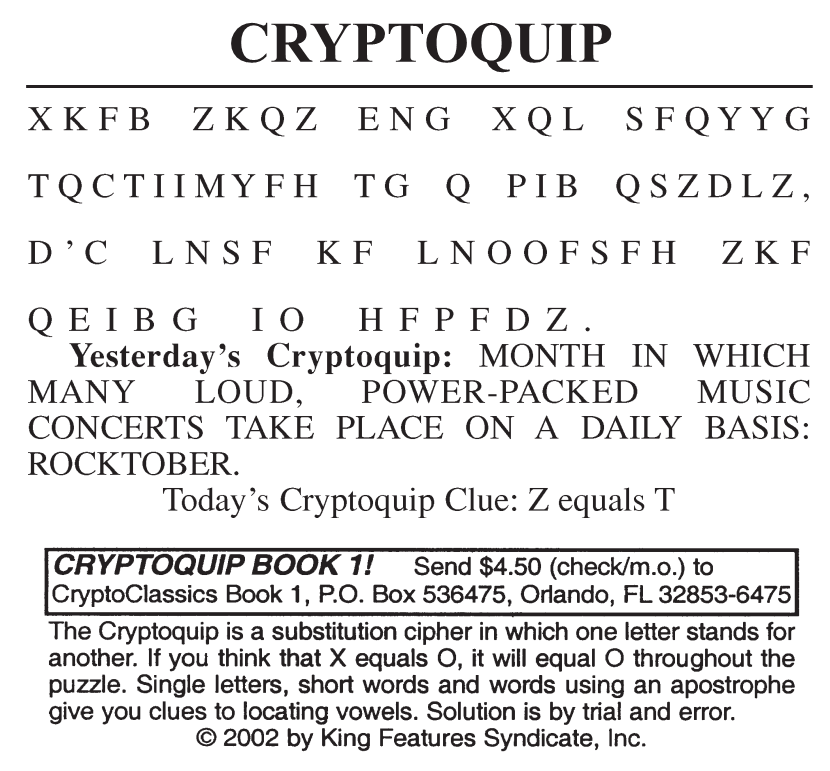
\includegraphics[width=3in]{images/cryptoquip.png}}
\caption{Example of cryptoquip (source: ``Cecil Whig'', \url{http://www.cecildaily.com/diversions/cryptoquip/ }).}
\label{fig:cryptoquip}
\end{figure}

\begin{exercise}
What is the total number of monoalphabetic cryptosystems?
\end{exercise}
Although there are many different possible monoalphabetic cryptosystems, they are relatively easy to break using frequency analysis. (You may even find web sites that can automatically decode cryptoquips.)


\subsection{Polyalphabetic codes}\label{subsec:polyCodes}

A cryptosystem would be more secure if a ciphertext letter could
represent more than one plaintext letter.  To give an example of this
type of cryptosystem, called a \term{polyalphabetic
cryptosystem},\index{Cryptosystem!polyalphabetic} we will generalize
affine codes by using matrices. The idea works roughly the same as
before; however, instead of encrypting one letter at a time we will
encrypt pairs of letters (as before, letters are represented by elements of ${\Bbb Z}_{26}$).  We can store a pair of letters $n_1$ and
$n_2$ in a vector  
$$
{\bold n} = 
\left(
\begin{array}{c}
n_1 \\ n_2
\end{array}
\right).
$$
Let $A$ be a $2 \times 2$ invertible matrix
with entries in ${\Bbb Z}_{26}$. We can define an encoding function by
$$
f({\bold n}) = (A \odot {\bold n}) \oplus {\bold b} ,
$$
where ${\bold b}$ is a fixed column vector and matrix operations are
performed in ${\Bbb Z}_{26}$. The formula for  the decoding function (which is the inverse of the encoding function) is very similar to the decoding function formula that we found for affine encoding:
$$
f^{-1}({\bold m}) = (A^{-1} \odot {\bold m}) \ominus (A^{-1} \odot {\bold b}),
$$
where $A^{-1}$ is the \emph{matrix inverse} of $A$: that is, $A^{-1}A = A A^{-1} = I$, where $I$ is the $2 \times 2$ identity matrix.  *Note* that in these formulas, we are using \emph{modular} matrix multiplication instead of \emph{regular} matrix multiplication: that is, the  regular $\cdot$ and $+$ operations are replaced by  $\odot$ and $\oplus$:

\begin{exercise}\label{exercise:crypt:mod_mult}
Perform the following operations using modular matrix multiplication (mod 26):
\begin{multicols}{2}
\begin{enumerate}[(a)]
\item
$\left(
\begin{array}{cc}
5 & 6 \\
7 & 8
\end{array}
\right)
\left(
\begin{array}{c}
4 \\
4
\end{array}
\right)$
\item
$\left(
\begin{array}{cc}
1 & 13 \\
16 & 2
\end{array}
\right)
\left(
\begin{array}{c}
3 \\
1
\end{array}
\right)$
\item
$\left(
\begin{array}{cc}
12 & 4 \\
13 & 5
\end{array}
\right)
\left(
\begin{array}{cc}
2 &1 \\
20 & 20 
\end{array}
\right)$
\item
$\left(
\begin{array}{cc}
13 & 2 \\
2 & 13
\end{array}
\right)
\left(
\begin{array}{cc}
2 &13 \\
13 & 2 
\end{array}
\right)$
\end{enumerate}
\end{multicols}
\end{exercise} 
 
\begin{example}\label{example:crypt:4}
Suppose that we wish to encode the word HELP. The corresponding
digit string is $7, 4, 11, 15$. If
$$
A =
\left(
\begin{array}{cc}
3 & 5 \\
1 & 2
\end{array}
\right),
$$
then
$$
A^{-1} 
=
\left(
\begin{array}{cc}
2 & 21 \\
25 & 3
\end{array}
\right).
$$
(You may check that $\bmod(AA^{-1},26) = \bmod(A^{-1}A,26) = I$.)
If ${\bold b} = \left( \begin{array}{c} 2 \\ 2 \end{array} \right)$, then our message is encrypted as
RRGR, where HE encrypts as RR and LP encrypts as GR.
\end{example}
In order to make use of polyalphabetic cryptosystems, we need to be able to find the inverse of a $2 \times 2$ matrix
with entries in ${\Bbb Z}_{26}$. As we *noted* above, this inverse is under matrix multiplication mod 26, rather than regular matrix multiplication.
Still, we can try to make use of the matrix inverse formula from regular matrix multiplication:
$$
\left( \begin{array}{cc} a & b \\ c & d \end{array} \right)^{-1}
= \frac{1}{ad-bc} \left( \begin{array}{cc} d & -b \\ -c & a \end{array} \right)  =  \left( \begin{array}{cc} kd & -kb \\ -kc & ka \end{array} \right),
$$
where 
$$ k = \frac{1}{ad - bc}.$$
This suggests that the following formula may be valid mod 26:
$$
\left( \begin{array}{cc} a & b \\ c & d \end{array} \right)^{-1}
=
\left( \begin{array}{cc} k \odot d & -k \odot b \\ -k \odot c & k \odot a \end{array} \right),
$$
where 
$$ k = ((a \odot d) \ominus (b \odot c))^{-1},$$
and $(\cdots)^{-1}$ means inverse under multiplication in ${\Bbb Z}_{26}$. 
We will see in the following exercise that  this works as long as $(a \odot d) \, \ominus \, (b \odot c)$ has a multiplicative inverse in ${\Bbb Z}_{26}$.

\begin{exercise}
Suppose that $(a \odot d) \, \ominus \, (b \odot c)$ has an inverse in ${\Bbb Z}_{26}$: that is to say, suppose there is a $k \in  {\Bbb Z}_{26}$ such that $k \odot ((a \odot d) \, \ominus \, (b \odot c)) = 1$.  Show that the matrices:
$$
A = \left( \begin{array}{cc} a & b \\ c & d \end{array} \right)~~~\text{and}~~~
B=
\left( \begin{array}{cc}  k \odot d & - k \odot b \\ - k \odot c &  k \odot a \end{array} \right)$$
are inverses of each other  in ${\Bbb Z}_{26}$.  That is, show that $AB = BA = I$ under matrix multiplication mod 26.

\end{exercise} 
The previous exercise leaves open the question of whether $\left( \begin{array}{cc} a & b \\ c & d \end{array} \right)$ has an inverse when $(a \odot d)  \ominus (b \odot c)$ has no inverse in ${\Bbb Z}_{26}$. Once again, we can reach back to our previous matrix knowledge to resolve this issue. Recall that the quantity $ad - bc$ is called the \term{determinant}\index{Matrix!determinant} of the matrix  $\left( \begin{array}{cc} a & b \\ c & d \end{array} \right)$.  There is also a famous formula for the determinant of the product of matrices:
$$\text{det}(A) \text{det}(B) = \text{det}(AB).$$
This same formula carries over to matrix multiplication mod 26, because (as we've seen) in any equation using only the operations of multiplication, addition, and subtraction, we can replace these operations with their modular versions and still have a true equation. We can use this to show that $(a \odot d)  \ominus (b \odot c)$ \emph{must} have an inverse in ${\Bbb Z}_{26}$ in order for $\left( \begin{array}{cc} a & b \\ c & d \end{array} \right)$ to have an inverse:

\begin{exercise}\label{exercise:crypt:mat1}
Suppose that $A = \left( \begin{array}{cc} a & b \\ c & d \end{array} \right)$ is a matrix with entries in ${\Bbb Z}_{26}$, such that  $(a \odot d)  \ominus (b \odot c)$ has no inverse in ${\Bbb Z}_{26}$. Show that $A$ has no inverse in  ${\Bbb Z}_{26}$.
\hyperref[sec:crypt:hints]{(*Hint*)}
\end{exercise}


\begin{exercise}\label{exercise:crypt:minv}
Find matrix inverses in ${\Bbb Z}_{26}$ for the following matrices. If no inverse exists, then prove there is no inverse.
\begin{multicols}{2}
\begin{enumerate}[(a)]
\item
$\left( \begin{array}{cc} 9 & 2 \\ 20 & 31 \end{array} \right)$
\item
$\left( \begin{array}{cc} 2 & 3 \\ 23 & 2 \end{array} \right)$
\item
$\left( \begin{array}{cc} 4 & 11 \\ 3 & 2 \end{array} \right)$
\item
$\left( \begin{array}{cc} 2 & 2 \\ 3 & 4 \end{array} \right)$
\end{enumerate}
\end{multicols}
\end{exercise}
 \begin{exercise}
For the same matrices as in Exercise~\ref{exercise:crypt:minv}, find the matrix inverses in ${\Bbb Z}_{29}$.
\end{exercise}

\begin{exercise}
Given that
$$
A =
\left(
\begin{array}{cc}
3 & 4 \\
2 & 3
\end{array}
\right),~~ \text{and~} {\bold b} = \left( \begin{array}{c} 2 \\ 5 \end{array}\right).$$
\begin{enumerate}[(a)]
\item
Use the encryption function $f({\bold p}) = A {\bold p} + {\bold b}$
to encode the message CRYPTOLOGY.  
\item
What is the decoding function?  
\end{enumerate}
 \end{exercise}
 
Frequency analysis can still be performed on a polyalphabetic
cryptosystem, because we have a good understanding of how pairs of
letters appear in the English language. The pair {\em th} appears
quite often; the pair {\em qz} never appears.  To avoid decryption by
a third party, we must use a larger matrix than the one we used in
Example~\ref{example:crypt:4}. 
  
\subsection{Spreadsheet exercises}
Spreadsheets can be used to automate many of the calculations that we have looked at in the previous sections.

\subsubsection*{Shift encoding and decoding spreadsheet \quad \sectionvideohref{6tgBvDI1Tiw&list=PL2uooHqQ6T7PW5na4EX8rQX2WvBBdM8Qo&index=35}}

\begin{exercise}\label{exercise:crypt:EngShift}
In this exercise, you will use a spreadsheet to create an automated shift encoder for English. Please refer to Figure~\ref{fig:AutoShiftEnc} for guidance:
\begin{figure}[h]
\center{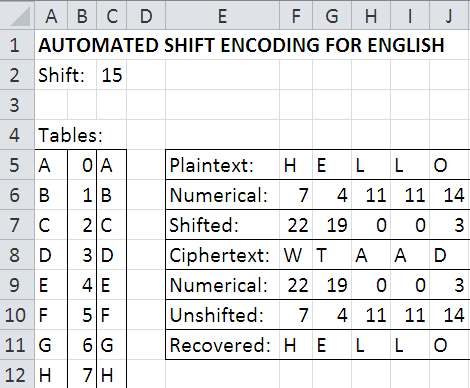
\includegraphics[width=3.0in]{images/AutoShiftEnc.png}}
\caption{Automatic shift encoder for English.}
\label{fig:AutoShiftEnc}
\end{figure}
\begin{enumerate}[(i)]
\item
Put the Shift value in cell C2.
\item
Put the alphabet (starting with A), numerical values for the letters (starting with 0), and the alphabet again in columns A, B, C starting on line 5.
\item
Type your plaintext in row 5, starting in column F.
\item
Row 6 beginning in column F contains the numerical values for the plaintext. The formula in cell F6 is: ``=VLOOKUP(F5, \$A\$5:\$B\$30,2)''. The significance of this formula is as follows:
\begin{itemize}
\item
The function VLOOKUP means that the program will look up a given value in a given table;
\item
The F5 is the first argument of VLOOKUP, which means that the value being looked up is in cell F5;
\item
The \$A\$5:\$B\$30 is the second argument of VLOOKUP, which means that it represents the cells containing the table that the value will be looked up in.  The dollar signs are used to guarantee that the table will remain fixed when the formula is copied and pasted into another cell;
The 2 which is the third lookup of VLOOKUP indicates that the value in the second column in the same row as the looked-up value is placed in the cell where the formula is located.
\end{itemize}
\item
Row 7 beginning in column F gives the encoded numerical values. The formula in cell F7 is ``=MOD(F6+\$C\$2,26)''.  The dollar signs on C2 guarantee that when the formula is copied, the shift still refers to the value in C2.
\item
Row 8 beginning in column F gives the ciphertext.  The formula in cell F8 is: ``=VLOOKUP(F7,\$B\$5:\$C\$30,2)''. 
\item
Rows 9,10, and 11 are similar to rows 6,7,8 respectively. Try to do this yourself. 
\end{enumerate}
Once you have completed the formulas, select cells F6 through J11, and use the spreadsheet's ``Fill Right'' capability to carry the formulas to the other columns.  (If your plaintext is longer, you can select more columns and fill right.
\end{exercise}

\begin{exercise}
The Spanish alphabet has 3 more letters than English:  `Ch' (comes after C in the alphabet), `Ll'  (comes after L in the alphabet), and `Nn' (comes after N).  Modify the sheet you created in Exercise \ref{exercise:crypt:EngShift} to make a Spanish language shift encoder.  Use your sheet to decode the following message:

MS KIUPVX	UIB NIKPS VX MB BPMUYAM MS UMQXA

(Note that `Ch' counts as a single letter.)
\end{exercise}

\subsubsection*{Affine encoding and decoding spreadsheet
\quad
\sectionvideohref{SJstRseE0V4&list=PL2uooHqQ6T7PW5na4EX8rQX2WvBBdM8Qo&index=34}}

\begin{exercise}
Create a spreadsheet that can perform any affine encoding on English plaintext.  You may model your spreadsheet on the sheet in Figure~\ref{fig:affine}.  Use your spreadsheet to decode the following message:


EMBNDOBFDZXIDPEMBSBJJJZOBFDZVOBUDSEVHOB

which was encoded using an affine encoding function with $b=21$.
\begin{figure}[h]
\center{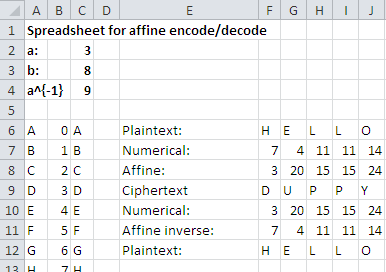
\includegraphics[width=3.5in]{images/Affine.png}}
\caption{Automatic affine encoder for English.}
\label{fig:affine}
\end{figure}
\end{exercise}

\begin{exercise}
In order to decode an affine cryptosystem on English letters with encoding function $f(p) = (a\odot p) \oplus b$, it is necessary to find the inverse of $a$ under multiplication mod 26. We have ways of finding inverses of individual numbers.  But we can also use spreadsheet software  to find all inverses in one fell swoop as described below.

Open a sheet in  your favorite spreadsheet software (Excel, LibreOffice, or OpenOffice). Put the numbers 0 through 25 in column A, starting at row 3, and also in row 2 starting in column B. To fill up the table, put the formula ``=MOD(\$A3*B\$2,26)'' in cell B3, as shown in Figure~\ref{fig:mod26mult}. This formula causes the software to take the product of the contents of cells A3 and B2, and put the result mod 26 into cell B3.  The dollar signs are important: these indicate ``fixed reference''.  For example, the `\$A3' means that when this formula is copied to other cells, the reference to column A remains unchanged while the column may change. On the other hand, the `B\$2' means that when the formula is copied to other cells, the reference to column 2 remains unchanged.

At this point, select the range of cells from B3 to AA28 (this will be a  square region of $26 \times 26$ cells. Use your spreadsheet's ``Fill down'' and ``Fill right'' feature to fill all the cells in this region. The location of all of the `1''s in this table shows all of the inverses.  For example, there is a '1' in the row labeled 9 and column labeled 3.  This means that 9 and 3 are inverses of each other mod 26.

Use this spreadsheet table to create a 2-column table: in the first column, put the numbers 0 through 26, and in the second column, put the inverses (if the number has no inverse, just put a `$-$').
\begin{figure}[h]
\center{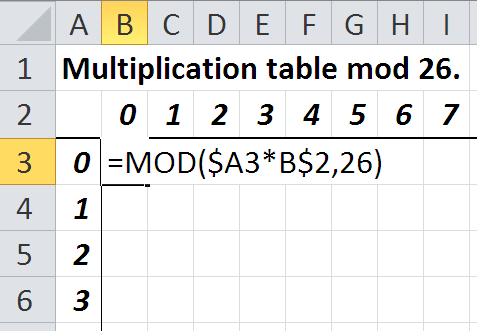
\includegraphics[width=2.25in]{images/MultMod26.png}}
\caption{Mod 26 multiplication table.}
\label{fig:mod26mult}
\end{figure}
\end{exercise}

\begin{exercise}
Following the previous exercise, find all inverses of the numbers mod 29 (this can be used in affine encoding of Spanish, which has 29 letters).
\end{exercise}

\begin{exercise}
Make a spreadsheet that can do polyalphabetic coding.  you may base your sheet's design on Figure~\ref{fig:polycrypto}. The figure shows the encoding of the word CRYPTOLOGY using 
$A = \left(
\begin{array}{cc}
3 & 5 \\
1 & 2
\end{array}
\right)$, and ${\bold b} = \left( \begin{array}{c} 2 \\ 2 \end{array}\right).$ 

Use your spreadsheet to decode the following words that were encoded using $f({\bold p}) = A {\bold p} + {\bold b}$ with the given $A$ and ${\bold b}$.
\begin{enumerate}[(a)]
\item
VVDGOFOKLY, $A= \left(
\begin{array}{cc}
13 & 5 \\
9 & 2
\end{array}
\right)$, and ${\bold b} = \left( \begin{array}{c} 7 \\ 13 \end{array}\right).$ 
\item
VWFGTWQKTA, $A= \left(
\begin{array}{cc}
17 & 13 \\
6 & 3
\end{array}
\right)$, and ${\bold b} = \left( \begin{array}{c} 14 \\ 18 \end{array}\right).$ 
\item
EXUFQPRRGA, $A= \left(
\begin{array}{cc}
3 & 4 \\
5 & 7
\end{array}
\right)$, and ${\bold b} = \left( \begin{array}{c} 4 \\ 8 \end{array}\right).$ 
\end{enumerate}
\begin{figure}[h]
\center{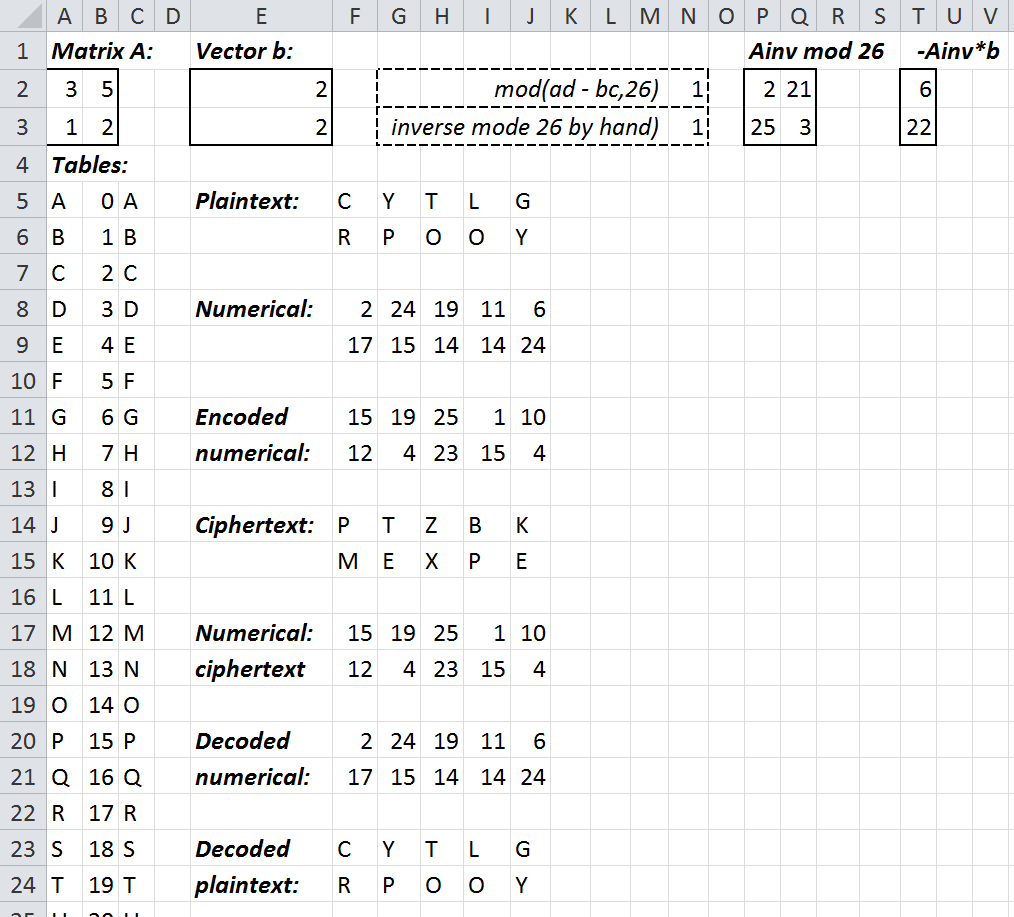
\includegraphics[width=5in]{images/polycrypto2.png}}
\caption{(Semi-)automatic polyalphabetic encoder/decoder for English. Note that cell N3 is entered by hand, based on the value in N2.}
\label{fig:polycrypto}
\end{figure}
\end{exercise}


\section{Public key cryptography}
\label{sec:publicKeyCrypto}
  
If traditional cryptosystems are used, anyone who knows enough to
encode a message will also know enough to decode an intercepted
message. In 1976, W.~Diffie\index{Diffie, W.} and
M.~Hellman\index{Hellman, M.} proposed public key cryptography, which
is based on the observation that the encryption and decryption
procedures need not have the same key. This removes the requirement
that the encoding key be kept secret. The encoding function $f$ must
be relatively easy to compute, but $f^{-1}$ must be extremely
difficult to compute without some additional information, so that
someone who knows only the encrypting key cannot find the decrypting
key without prohibitive computation. It is interesting to note that to
date, no system has been proposed that has been proven to be
``one-way;'' that is, for any existing public key cryptosystem, it has
never been shown to be computationally prohibitive to decode messages
with only knowledge of the encoding key. 
 
 
 
\subsection{The RSA cryptosystem\quad
\sectionvideohref{NPA_Q0M4n54&list=PL2uooHqQ6T7PW5na4EX8rQX2WvBBdM8Qo&index=37}}\label{sec:RSA}
 
The RSA cryptosystem introduced by R.~Rivest\index{Rivest, R.},
A.~Shamir\index{Shamir, A.}, and L.~Adleman\index{Adleman, L.} in
1978, is based on the difficulty of factoring large numbers. Though it
is not a difficult task to find two large random primes and multiply
them together, factoring a 150-digit number that is the product of two
large primes would take 100 million computers operating at 10 billion
instructions per second about 50,000 years under the fastest
algorithms currently known.
 
Let us look at how RSA works in a practical context.  
Suppose that Jennifer is running an online boutique, and wants to receive
 credit card information from customers over the internet. Unfortunately it's all too easy to snoop the internet, 
and it certainly wouldn't be good for Jennifer's customers if their credit card numbers were stolen. 
So she needs a suitable code for the credit card information in order to protect her customer's privacy.
The code may be constructed as follows:
\begin{enumerate}[(a)]
\item 
Choose  two random 150-digit prime
numbers $p$ and $q$. (This is easier said than done!  We will consider some possible ways of doing this in Section~\ref{primality}.)
\item
Compute the product $n= pq$ as well as $ m = (p - 1)(q-1)$. 
(It can be shown that $m$ is actually the number of positive integers in $\mathbb{Z}_n$ that are relatively prime to $n$.)    
\item
Find a large random integer $E$ that is relatively prime to $m$. This is done by making a guess for $E$, then using the Euclidean algorithm to check whether $\gcd(E, m) = 1$. If not, then keep guessing until you find an $E$ that works. In general relatively prime numbers are not uncommon, and the Euclidean algorithm is pretty quick (especially for a computer), so $E$ is not too difficult to find.  
\item
Using the Euclidean algorithm, find $D$ such that $\mbox{DE} \equiv 1 \pmod{m}$. 
\end{enumerate}
 Now, let's say that Jennifer has a  customer whose credit card number is $x$.  Before requesting the credit card information, Jennifer's computer  sends the numbers  $E$ and $n$ to the customer's computer, which then calculates $y = x^E \mod n$ and sends $y$ to
Jennifer's computer, Jennifer recovers $x$ by computing  $y^D \bmod
n$, which (as we shall show in a minute) turns out to be $x$, as long as $x$ is less than $n$. 

Notice some amazing things here. First, $E$ and $n$ are sent out \emph{openly} over the internet. Jennifer doesn't care if  snoopers find out this information. In fact, she sends the \emph{same} $E$ and $n$ to each customer! But this does not compromise her customers' security, because only Jennifer knows $m$, and it takes both $E$ and $m$ to find $D$. As long as no one can figure out $m$, the credit card numbers are safe!

To summarize: once the public key $(E,n)$ and the private key $D$ have been constructed, the process of encoding and decoding is simple:
\begin{itemize}
\item
To encode a numerical plaintext $x$:  compute $\mod (x^E,n)$ .
\item
To decode a numerical ciphertext $y$: compute $\mod(y^D,n)$.
\end{itemize}
 
\vspace{2 ex}
 
\begin{example}
Before exploring the theory behind the RSA cryptosystem or attempting
to use large integers, we will use some small integers just to see
that the system does indeed work. Suppose that we wish to send some
message, which when digitized is 395. Let $p = 23$ and $q = 29$.  Then 
$$ n = pq = 667 \qquad \textrm{and} \qquad
m = (p - 1)(q - 1) = 616.
$$
We can let $E = 487$, since $\gcd(616, 487) = 1$. The encoded message
is computed to be  
$$
\bmod(395^{487},  667) = 570.
$$
(This may seem like a very long computation, but there are fast ways of doing this: see Exercise \ref{exercise:crypt:power} below.)
Using the Euclidean
algorithm, we determine that $191 E = 1 + 151 m$; therefore, the
decrypting key is $(n, D) = ( 667, 191)$. We can recover the original 
message by calculating  
$$
 \bmod(570^{191}, 667) = 395.
$$
\end{example}
 
 
\vspace{ 2 ex}
 
 
This really seems like magic. How in the world does it work? 
First of all, we know that $DE
\equiv 1 \bmod{ m}$; so there exists a $k$ such that 
$$
DE = km + 1.
$$
This means that
$$
y^D = (x^E)^D = x^{DE} = x^{km+1} = (x^m)^k x.
$$
At this point we need \emph{Euler's theorem} from Chapter~\ref{cosets}, which states the following. Suppose $m$ is the number of positive integers less than $n$ that are relatively prime to $n$. Then it is true that:
$$
x^m \equiv 1 \pmod n.
$$
for \emph{any} $x$ that is relatively prime to $n$. 

We can use this to simplify our previous expression for $y^D$:
$$
y^D =  (x^m)^k x \equiv (1)^k x  \equiv x \bmod n,
$$
 and presto! We have our result.
 
We can now ask how one would go about breaking the RSA cryptosystem.
To find $D$ given $n$ and $E$, we simply need to factor $n$ and solve
for $D$ by using the Euclidean algorithm. If we had known that $667 =
23 \cdot 29$ in Example~5, we could have recovered $D$.    
 
 
 
\begin{exercise}\label{exercise:crypt:primes}
Show that if $p$ and $q$ are primes, then the number of positive integers less than $pq$ which are relatively prime to $pq$ is $(p-1)(q-1)$.
\hyperref[sec:crypt:hints]{(*Hint*)}
\end{exercise}
 
\subsection{Message verification}\label{crypt:verify}
 
 
There is a problem of message verification in public key
cryptosystems. Since the encoding key is public knowledge, anyone has
the ability to send an encoded message.  If Alice receives a message
from Bob, she would like to be able to verify that it was Bob who
actually sent the message. Suppose that Bob's encrypting key is $(n',
E')$ and his decrypting key is $(n', D')$.  Also, suppose that Alice's
encrypting key is $(n, E)$ and her decrypting key is $(n, D)$.  Since
encryption keys are public information, they can exchange coded
messages at their convenience.  Bob wishes to assure Alice that the
message he is sending is authentic. Before Bob sends the message $x$
to Alice, he decrypts  $x$ with his own key:
$$
x' =  \bmod(x ^{D'}, n').
$$
Anyone can change $x'$ back to $x$ just by encryption, but only Bob
has the ability to form $x'$. Now Bob encrypts $x'$ with Alice's
encryption key to form 
$$
y' = \bmod({x'}^E,   n),
$$
a message that only Alice can decode.  Alice decodes the message and
then encodes the result with Bob's key to read the original message, a
message that could have only been sent by Bob.
 

\subsection{RSA exercises\quad
\sectionvideohref{1f2C9LXTIRg&list=PL2uooHqQ6T7PW5na4EX8rQX2WvBBdM8Qo&index=38}}
 

\begin{exercise}\label{exercise:crypt:power}
This problem demonstrates a fast method for computing very large powers of numbers in modular arithmetic using a spreadsheet.  You will need this method in order to do the subsequent problems. We will demonstrate the method by computing $\bmod(23^{485} ,617)$.
\begin{enumerate}[(a)]
\item
Use a spreadsheet to compute the following sequence of numbers:
\[ 23, \bmod(23^2 ,617),\bmod(23^4 ,617),\ldots,\bmod(23^{256} ,617) \]
Note that each power of 23 in this series is the  \emph{square} of the previous power.  So to compute any number in this series, square the previous number and reduce mod 617.  You may use the MOD spreadsheet function.  It is easiest to put all the numbers in a single column. (This way, you can use the spreadsheet's ``Fill down'' feature.)
\item  Write 485 as a sum of powers of 2.  (This is the same thing as finding the \emph{binary expansion} of 485.)
\item Using the results of (b), identify a set of entries from the table you found in part (a), such that the product of these entries is equivalent to $23^{485}  \pmod{617}$.
\hyperref[sec:crypt:hints]{(*Hint*)}
\item 
Use your result from (c) to compute $\bmod(23^{485} ,617)$.
\end{enumerate}
\end{exercise}

\begin{exercise}\label{exercise:crypt:powerplus}
Building off the previous exercise, create a spreadsheet that can compute $\bmod(x^{q},n)$ for general $x,q,n$.  You may follow the pattern of the spreadsheet in Figure~\ref{fig:LargePowMod}.  Some of the formulas in the spreadsheet are:
\begin{itemize}
\item
Cell A8: ~~=B3
\item
Cell B8: ~~=MOD(A8,2)
\item
Cell A9: ~~=(A8 - B8)/2
\item
Cell D9: ~~ = D8*2
\item
Cell E9: ~~ = MOD(E8*E8, \$B\$4)
\item
Cell F8: ~~ = B8
\item
Cell G8: ~~ = E8$\widehat{~~}$F8
\item
Cell H8: ~~ = G8
\item
Cell H9: ~~ = MOD(G9*H8,\$B\$4)
\end{itemize}
You may obtain the rest of the formulas using the spreadsheet's ``fill down'' capability.

\begin{figure}[h]
\center{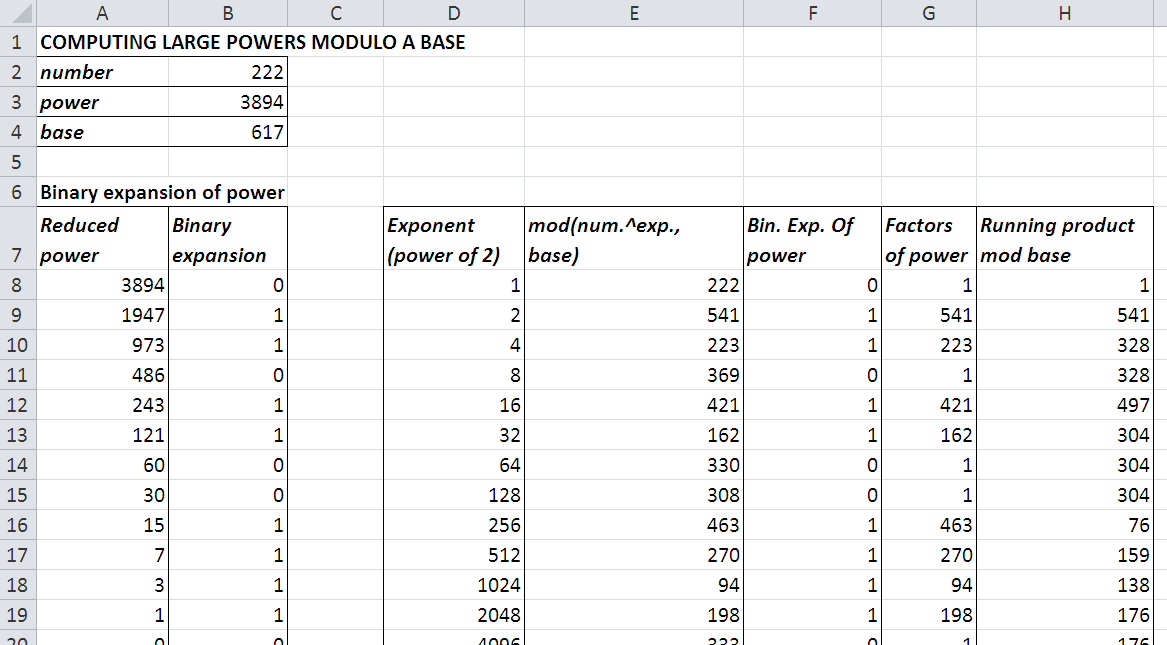
\includegraphics[width=5.5in]{images/LargePowMod.png}}
\caption{Spreadsheet for taking large powers modulo a given base.}
\label{fig:LargePowMod}
\end{figure}
\end{exercise} 


\begin{exercise}\label{exercise:crypt:RSA_E}
Using your spreadsheet from the previous exercise, encrypt each of the following plaintexts using RSA. Before encoding, divide the plaintext
into blocks of integers of length 2;  that is, if the plaintext is $142528$, encode 
14, 25, and 28 separately.
 
\begin{enumerate}[(a)]
  \item
$n = 3551, E = 629$, plaintext = 31
 \item
$n = 2257, E = 47, $ plaintext  = 23
 \item
$n = 120979, E = 13251,$ plaintext = 142371
\item
$n = 45629, E = 781,$ plaintext = 231561
 
\end{enumerate}
\end{exercise}
 
\begin{exercise}\label{exercise:crypt:RSA_D}
Decrypt each of the following RSA messages $y$. (In this case, do not break $y$ into blocks--decode the entire number.)
 
 \begin{enumerate}[(a)]
\item
 $n = 3551, D = 1997, y = 2791$
 \item
$n = 5893, D = 81, y = 34$
 \item
$n = 120979, D = 27331, y = 112135$
 \item
$n = 79403, D = 671, y = 129381$
 \end{enumerate}
 \end{exercise}
 
%\begin{exercise}
%For each of the following encryption keys $(n, E)$ in the RSA
%cryptosystem, compute $D$.(\emph{Hint}
% 
%\vspace{3pt}        %two column exercise list
% 
%\hspace{-7pt}
%\begin{minipage}[t]{4.6in}
%\noindent
%\begin{minipage}[t]{2.25in}
%\begin{itemize}
% 
% \item[{\bf (a)}]
%$(n, E) = (451, 231)$
% 
% \item[{\bf (c)}]
%$(n, E) = (37986733, 12371)$
% 
%\end{itemize}
%\end{minipage} \hfill
%\begin{minipage}[t]{2.25in}
%\begin{itemize}
% 
% \item[{\bf (b)}]
%$(n, E) = (3053, 1921)$
% 
% \item[{\bf (d)}]
%$(n, E) =\\ (16394854313, 34578451)$
% 
%\end{itemize}
%\end{minipage}
%\end{minipage}
% 
%\vspace{2pt}        %end two column exercise list
% \end{exercise}
 
\begin{exercise} 
Encrypted messages are often divided into blocks of $n$ letters. A
message such as THE WORLD WONDERS WHY might be encrypted as 
JIW OCFRJ LPOEVYQ IOC but sent as JIW OCF RJL POE VYQ
IOC.  What are the advantages of using blocks of $n$ letters? 
 \end{exercise}
 
 
\begin{exercise}
Construct an RSA cryptosystem as follows:
\begin{enumerate}[(a)]
\item
On the web, find two four-digit primes
\item
Use these primes to compute $n$ and $m$.
\item
Choose a value of $E$ which is less than $m$, and use you Diophantine Equation spreadsheet (Exercise~\ref{exercise:modular:DiophantineSS} in the Modular Arithmetic chapter) to find the inverse $D$ under multiplication mod $m$.  If it turns out that $E$ is not relatively prime to $m$, try again.
\item
Test your cryptosystem by encoding `123', and then decoding it. To encode, use the spreadsheet that you 
created in Exercise~\ref{exercise:crypt:powerplus} earlier in this chapter. To decode, make another copy of the same sheet.
\end{enumerate}
\end{exercise} 
 
 
\subsection{Additional exercises: identifying prime numbers\quad
\sectionvideohref{h971dgcV5-0&list=PL2uooHqQ6T7PW5na4EX8rQX2WvBBdM8Qo&index=36}}\label{primality}
 
We saw in Section~\ref{sec:RSA} that the RSA algorithm depends on finding very large primes. In practice, large primes are found using trial and error. That is, we choose a large random number and test to see whether it's prime. 
If the test fails, then try, try again.

So it all comes down to figuring out how to test whether a number is prime. In this section, we consider some possible ways of doing this.

\subsubsection*{\emph{``Brute force'' method, and sieve of Eratosthenes}}
On way to do this is sheer brute force: try dividing by 2,3,4, $\ldots$, and if nothing divides then the number is prime. There are various ways to make this process more efficient, as we will see in the following exercises.

\begin{exercise}\label{exercise:crypt:brute}
To test whether the number $n$ is a prime, you divide $n$ all the integers $1,2,3, \dots$ up to $a$, and see if any of them divides evenly.  How large does $a$ have to be in order to guarantee that $n$ really is a prime?
\hyperref[sec:crypt:hints]{(*Hint*)}
\end{exercise}

When testing whether $n$ is prime, by the ``brute force'' method, as long as $n$ is odd we don't need to divide by even numbers (Why?). 
This means that you only need to test about half of the numbers up to $a$--more precisely, we only need to test $\lceil a/2 \rceil$ numbers, where $\lceil x \rceil$ means ``the next integer larger than $x$''. ($\lceil x \rceil$ is called the \emph{ceiling} of $x$.\index{Ceiling!of a real number}) 

We can pull the same trick with factors that are divisible by 3.  Once we've tested 3 as a factor, we don't need to check $9, 15, 21, \ldots$ or any other number that is divisible by 3.  (Why?)  So it seems that this reduces the number of factors that we need to check by about a third, since every third integers are divisible by 3. However, we need to be careful here. We've already ruled out the numbers that are divisible by 2, so the numbers that are divisible by both 2 and 3 have already been ruled out. In other words (using $m$ to denote a positive integer, and using the the notation $| \{ \cdots \} |$ to denote the size of sets):
\begin{align*}
&| \{ m \le a \text{ and } (2 \mid m \text{ or } 3 \mid m) \}| =\\ 
&~~~| \{ m \le a  \text{ and } 2 \mid m \}| + | \{ m \le a  \text{ and } 3 \mid m \}| - | \{ m \le a  \text{ and } 6 \mid m \}|.
\end{align*}
If we are not so careful with the ``ceiling function'' (which changes the result by at most 1 anyway), this tells us:
\begin{align*}
| \{ m \le a \text{ and } 2 \mid m \text{ or } 3 \mid m \}| &\approx 
\frac{a}{2} + \frac{a}{3} -\frac{a}{6}.
\end{align*}
We can turn this around and find the number of integers which are \emph{not} divisible by 2 or 3:
\begin{align*}
| \{ m \le a \text{ and } 2 \nmid m \text{ and } 3 \nmid m \}| &\approx 
a - \frac{a}{2} - \frac{a}{3} + \frac{a}{6} \\
&\approx a\left(1 - \frac{1}{2}\right) \left(1 - \frac{1}{3}\right)\\
&\approx \frac{a}{3}.
\end{align*}
This gives the number of trial divisions required to test whether $n$ is prime. (Of course we also need to test divisibility by 2 and 3, which are 2 additional divisions.)

The same reasoning can be extended to take into account divisibility by 5, 7, 11, and so on:

\begin{exercise}\label{exercise:crypt:EulerTotient}
Using the same reasoning as above, show that after dividing by $2,3,5$ the number of additional divisions required to test for primality is approximately:
$$a\left(1 - \frac{1}{2}\right) \left(1 - \frac{1}{3}\right)\left( 1 - \frac{1}{5} \right).$$
\end{exercise}

The technique of eliminating numbers to check based on previous divisibility is called the \term{sieve of Eratosthenes}\index{Sieve of Eratosthenes}.


\subsubsection*{\emph{Fermat's test for primality}}
Even using various tricks to reduce the number of computations, the brute force method requires far too many calculations to be useful for RSA encoding. A different algorithm for testing primality is \term{
Fermat's factorization algorithm}\index{Fermat!factorization
algorithm}, which depends on the following fact:

\begin{exercise}\label{exercise:crypt:Fermat}
Let $n= ab$ be an odd composite number. Prove that $n$ can be written
as the difference of two perfect squares :
$$
n = x^2 - y^2 = (x-y)(x+y),
$$
where both $x$ and $y$ are greater than 1. Consequently, a positive odd integer can be factored exactly when we
can find integers $x$ and $y$ such that $n = x^2 - y^2$.
\hyperref[sec:crypt:hints]{(*Hint*)} 
\end{exercise} 
We can use this fact to factor $n$ by trying different pairs of squares in order to get $n$ as the difference of the two.  Of course, we want to do this systematically. So we want to see what values of $x$ and $y$ we actually need to check:

\begin{exercise}\label{exercise:crypt:smallest_value}
In the formula  $n = x^2 - y^2 = (x-y)(x+y)$,  what is the smallest possible value for $x$ that needs to be tested?
\hyperref[sec:crypt:hints]{(*Hint*)}
\end{exercise}

There are other special conditions that $x$ and $y$ must satisfy:

\begin{exercise}\label{exercise:crypt:FermatEfficient}
\begin{enumerate}[(a)]
\item
Assuming that $n$ is an odd number, show that if $x$ is odd then $y$ is even, and if $x$ is even then $y$ is odd.
\hyperref[sec:crypt:hints]{(*Hint*)}
\item
Show that for any odd number $m$, then $\mod(m^2,4) = 1$.
\hyperref[sec:crypt:hints]{(*Hint*)}
\item
Let $m = x + y$. Show that $m$ is odd, and that we can rewrite  $n  = (x-y)(x+y)$ as: $n = m(m-2y)$. 
\item
Show that if $\mod(n,4)=1$, then $y$ must be even.
\hyperref[sec:crypt:hints]{(*Hint*)}
\item
Show that if $\mod(n,4)=3$, then $y$ must be odd.
\hyperref[sec:crypt:hints]{(*Hint*)}
\end{enumerate}
\end{exercise}

The Fermat primality testing scheme is better for finding factors that are nearly equal. The brute force method of Exercise~\ref{exercise:crypt:brute}  is much better when one factor is much bigger than the other one.

\begin{exercise}\label{exercise:crypt:brute}
\begin{enumerate}[(a)]
\item
Create a spreadsheet that factors large numbers using the brute force scheme. You may use the spreadsheet in Figure~\ref{fig:bf} for inspiration. Some of the formulas in the spreadsheet are:
\begin{itemize}
\item
Cell A7: ~~=A6+2
\item
Cell B6:  ~~=\$B\$2/A6
\item
Cell C6:  ~~=IF(B6=FLOOR(B6,1),A6,0)
\item
Cell E2: ~~=MAX(C6:C99999)
\end{itemize}
You may obtain the rest of the formulas using the spreadsheet's ``fill down'' capability.
\item
Use this spreadsheet to factor $n=3551$. Then, use your result to find the decoding key $D$ for Exercise~\ref{exercise:crypt:RSA_E} part (a).
\item
Use this spreadsheet to  find the decoding key $D$ for Exercise~\ref{exercise:crypt:RSA_E} part (b).
\item
Use this spreadsheet to  find the decoding key $D$ for Exercise~\ref{exercise:crypt:RSA_E} part (c).
\item
Use this spreadsheet to  find the decoding key $D$ for Exercise~\ref{exercise:crypt:RSA_E} part (d).
\item
Given the encryption key $(n,E) = (451,231)$, find $D$.
\item
Given the encryption key $(n,E) = (3053,1921)$, find $D$.
\end{enumerate}
\end{exercise}

\begin{figure}[h]
\center{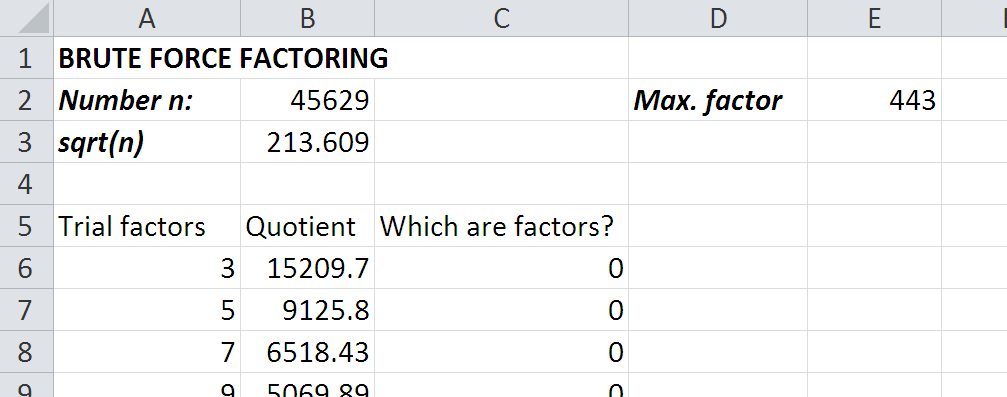
\includegraphics[width=4in]{images/bf.png}}
\caption{Spreadsheet for brute force factoring method}
\label{fig:bf}
\end{figure}


\begin{exercise}\label{exercise:crypt:FermatSpreadsheet}
\begin{enumerate}[(a)]
\item
Make a spreadsheet for Fermat's factoring method. You may use the spreadsheet in Figure~\ref{fig:FermaFact} for inspiration. Some of the formulas in the spreadsheet are:
\begin{itemize}
\item
Cell A7: ~~=A6+1
\item
Cell B6:  ~~=SQRT(A6*A6 - \$B\$2)
\item
Cell C6:  ~~=IF(B6=FLOOR(B6,1),A6-B6,0)
\item
Cell D6:  ~~=IF(B6=FLOOR(B6,1),A6+B6,0)
\item
Cell E2: ~~=MAX(C6:C99999)
\item
Cell E3: ~~=MAX(D6:D99999)
\end{itemize}
You may obtain the rest of the formulas using the spreadsheet's ``fill down'' capability.
\item
Use this spreadsheet to factor $n=7433551$. Then, use your result to find the decoding key $D$ for $(n,E) = (7433551,12345)$.
\item
Use this spreadsheet to factor $n=16394854313$. Then, use your result to find the decoding key $D$ for $(n,E) = (16394854313,34578451)$. 
\end{enumerate}
\end{exercise}


\begin{figure}[h]
\center{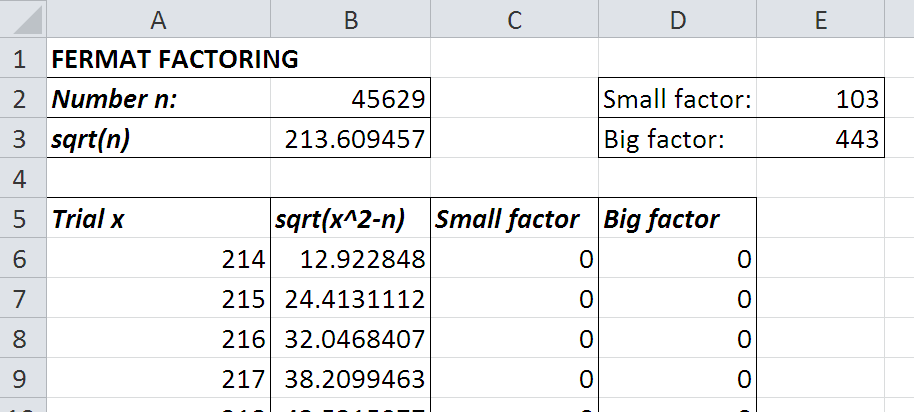
\includegraphics[width=4in]{images/FermaFact.png}}
\caption{Spreadsheet for Fermat difference-of-squares factoring method}
\label{fig:FermaFact}
\end{figure}

\begin{exercise}
* Using the results from Exercise~\ref{exercise:crypt:FermatEfficient} parts (d) and (e), modify the spreadsheet that you created in Exercise~\ref{exercise:crypt:FermatSpreadsheet} to make it twice as efficient.  In other words, modify the formula in cell A6 so that you can replace the formula in A7 with the formula: `=A6+2'.
\end{exercise}

\subsubsection*{\emph{Probabilistic methods using the ``little Fermat theorem''}}
In practice, neither the brute force nor the Fermat method is used to verify large prime numbers. Instead, 
\emph{probabilistic methods} are used: these methods can show that it's very, very likely that $n$ is a prime, but they don't prove for certain. The principal test of this type is the  \term{Miller-Rabin test} for primality. \index{Prime!Miller-Rabin test for} This test uses some of the principles described  below.	 
 
In Exercise~\ref{exercise:cosets:FermatLittle} in Section~\ref{sec:Fermat}, we will prove the following fact (which is widely known as \emph{Fermat's little theorem}\index{Fermat!little theorem}): 
\medskip

If  $p$ is any prime number and $a$ is any nonzero integer, then $a^{p-1} \equiv 1 \pmod{p}$.  
\medskip

We can use Fermat's little theorem as a screening test for primes. For example, 15 cannot be prime since
$$
2^{15-1} \equiv 2^{14} \equiv 4 \pmod{15}.
$$
However, 17 is a potential prime since
$$
2^{17-1} \equiv 2^{16} \equiv 1 \pmod{17}.
$$
We say that an odd composite number $n$ is a \term{
pseudoprime}\index{Pseudoprime} if 
$$
2^{n-1} \equiv 1 \pmod{n}.
$$

\begin{exercise}\label{exercise:crypt:prime_pseudo}
Which of the following numbers are primes  and which are pseudoprimes?
  
\vspace{3pt}        %two column exercise list
 
\hspace{-7pt}
\begin{minipage}[t]{4.6in}
\noindent
\begin{minipage}[t]{2.25in}
\begin{itemize}
 
 \item[{\bf (a)}]
341
 
 \item[{\bf (c)}]
601
 
 \item[{\bf (e)}]
771
 
\end{itemize}
\end{minipage} \hfill
\begin{minipage}[t]{2.25in}
\begin{itemize}
 
 \item[{\bf (b)}]
811
 
 \item[{\bf (d)}]
561
 
 \item[{\bf (f)}]
631
 
\end{itemize}
\end{minipage}
\end{minipage}
 
\vspace{2pt}        %end two column exercise list
\end{exercise} 
 
Let $n$ be an odd composite number and $b$ be a positive integer such
that $\gcd(b, n) = 1$. If $b^{n-1} \equiv 1 \pmod{n}$, then $n$ is a
\term{pseudoprime base} $b$. We can get a more accurate test for the  primality of $n$  if we 
test $n$ versus a number of prime bases. If $n$ is a pseudoprime for several prime bases, then we can say with high confidence that $n$ is most probably a prime.


\begin{exercise}
Show that 341 is a pseudoprime base 2 but
not a pseudoprime base 3.
\end{exercise}  

There exist composite numbers that are pseudoprimes for all bases to
which they are relatively prime.  These numbers are called \term{
Carmichael numbers}\index{Carmichael numbers}. The first Carmichael
number is $561 = 3 \cdot 11 \cdot 17$.  In 1992, Alford, Granville, and
Pomerance proved that there are an infinite number of Carmichael
numbers [4].  However, Carmichael numbers are very rare.  There are
only $2163$ Carmichael numbers less than $25 \times 10^9$. For more
sophisticated primality tests, see [1], [6], or [7].  
 
 
\begin{rem} (\emph{historical background})   Encrypting secret messages goes as far back as ancient Greece and
Rome. As we know, Julius Caesar used a simple shift code to send and
receive messages. However, the formal study of  encoding and decoding
messages probably began with the Arabs in the 1400s. In the fifteenth
and sixteenth centuries mathematicians such as Alberti and Viete
discovered 
that monoalphabetic cryptosystems offered no real security. In the
1800s, F. W. Kasiski established methods for breaking ciphers in
which a ciphertext letter can represent more than one plaintext
letter, if the same key was used several times. This discovery led to
the use of cryptosystems with keys that were used only a single time.
Cryptography was placed on firm mathematical foundations by such people
as W. Friedman and L. Hill in the early part of the twentieth century.
 
 
During World War II mathematicians were very active in cryptography.
Efforts to penetrate the cryptosystems of the Axis nations were 
organized in England and in the United States by such notable
mathematicians as Alan Turing and A. A. Albert. The period after
World War I saw the development of special-purpose machines for
encrypting and decrypting messages. The Allies gained a 
tremendous advantage in World War II by breaking the ciphers produced by 
the German Enigma machine and the Japanese Purple ciphers.
 
 
By the 1970s, interest in commercial cryptography had begun to take
hold. There was a growing need to protect banking transactions,
computer data, and electronic mail. In the early 1970s, IBM developed
and implemented LUZIFER, the forerunner  of the National Bureau of
Standards' Data Encryption Standard (DES). 
 
 
The concept of a public key cryptosystem, due to Diffie and Hellman,
is very recent (1976). It was further developed by Rivest,  
Shamir, and Adleman with the RSA cryptosystem (1978). It is not known
how secure any of these systems are. The trapdoor knapsack
cryptosystem, developed by Merkle and Hellman, has been broken. It is
still an open question whether or not the RSA system can be broken. As of 2014, 360-digit numbers 
have been factored--in practice, RSA keys of more than 1000 digits may be used.

There's been a great deal of controversy about research in
cryptography in recent times: the National Security Agency would like to
keep information about cryptography secret, whereas the academic community
has fought for the right to publish basic research.   
What's not controversial is that cryptography has come a long way since 1929, when Henry Stimson, 
Secretary of State under Herbert Hoover, dismissed the Black Chamber
(the State Department's cryptography division) in 1929 on the ethical 
grounds that ``gentlemen do not read each other's mail.''
\end{rem} 
 
\section{References and suggested readings}
\label{sec:References}
 
{\small
\begin{itemize}
 
\item[{\bf [1]}]
Bressoud, D. M. {\it Factorization and Primality Testing}.
Springer-Verlag, New York, 1989. 
 
\item[{\bf [2]}]
Diffie, W. and Hellman, M. E. ``New Directions in
Cryptography,'' {\it IEEE Trans. Inform. Theory} {\bf
22} (1976), 644--54.
 
\item[{\bf [3]}]
Gardner, M. ``A New Kind of Cipher that Would Take a Million
Years to Break,'' {\it Scientific American} {\bf
237} (1977), 120--24.
 
\item[{\bf [4]}]%%%%%%%%%%%%%%checked
Granville, A. ``Primality Testing and Carmichael Numbers,'' {\it
Notices of the American Mathematical Society} {\bf 39}(1992),
696--700. 
 
 
 
\item[{\bf [5]}]
Hellman, M. E. ``The Mathematics of Public Key
Cryptography,''  {\it Scientific American} {\bf 241}
(1979), 130--39.
 
\item[{\bf [6]}]%%%%%%%%%%%%%%checked
Koblitz, N. {\it A Course in Number Theory and Cryptography}.
Springer-Verlag, New York, 1987. 
 
 
\item[{\bf [7]}]
Pomerance, C., ed. {\it Cryptology and Computational Number
Theory}. Proceedings of Symposia in Applied Mathematics,
vol. 42. American Mathematical Society, Providence, RI,
1990.
 
 
\item[{\bf [8]}]
Rivest, R. L., Shamir, A., and Adleman, L., ``A Method for
Obtaining Signatures and Public-key Cryptosystems,'' {\it
Comm. ACM} {\bf 21}(1978), 120--26.
 
\end{itemize}
}
%%%%(c)
%%%%(c)  This file is a portion of the source for the textbook
%%%%(c)
%%%%(c)    Abstract Algebra: Theory and Applications
%%%%(c)    Copyright 1997 by Thomas W. Judson
%%%%(c)
%%%%(c)  See the file COPYING.txt for copying conditions
%%%%(c)
%%%%(c)
\chap{Further topics in Cryptography}{Crypto}
\section{Diffie Hellman Key Exchange}\label{sec:DHKE:1}

In order to share a private message over a public domain a sender must  "lock" or encrypt their message using a \emph{key}\index{key! in cryptogaphy}.  Recall from Section \ref{sec:crypt:overview}, that in cryptography a  key is a special piece of information (usually a number)  that is required to encrypt and decrypt data which is shared between the sender and receiver. There are generally three types of keys used: public, private and symmetric keys. A \emph{Public Key}\index{Public Key! in cryptography} can be widely distributed, and is used for encrypting messages.  A\emph{Private Key}\index{Private Key! in cryptography} is only known to the sender, and is used for decrypting messages (it can also be used for encrypting messages when using cryptosystems such as RSA).  Finally, a \emph{Symmetric Key}\index{Symmetric Key! in cryptography} is known by the sender and receiver, and is used to encypt and decrypt messages.  Not all cryptosystems require all three kinds of keys, but every cryptosystem must have either a private key or a symmetric key.

  If a symmetric key is used, then both parties must share their key before they can begin communicating securely. The requirement of establishing a key exchange is so essential that it is embedded into almost every technology we use today.  Some examples of key exchange can be seen in media applications, cell phones, banking, online purchasing, and emails.  

 But what if the only way the two parties have to communicate is via a public network (such as the Internet), where eavesdroppers can listen in?  Under these conditions how can they possibly establish a shared key in such a way that no one else can find out?  The Diffie Hellman Key Exchange (DHKE) is one possible solution to the problem of creating a secret key over an insecure communication channel.  Note that the DHKE is not used for encryption/decryption of messages, but only to establish a key that can be used to encrypt/decrypt subsequent messages.  Follow the steps below to see the DHKE process.  

 \begin{enumerate}[Step 1.]
 \item First, Moses and Rachael agree upon a pair of numbers $p$ and $g$. $p$ is called the \term{modulus},while $g$ is called the \term{base}. These numbers are not secret, and Moses and Rachael don't care if eavesdroppers find out what $p$ and $g$ are. In practice $p$ and $g$ are required to have certain properties (as explained below) to maximize secrecy.  However, the DHKE procedure still works for any values of $p$ and $g$.
\item Moses chooses a secret integer $n$, known only to himself.  He then computes $q$ where $q =\bmod(g^n,p)$, and sends Rachael the value of $q$. Rachael does not need to know the value of $n$.
\item Rachael similiarly chooses her own secret integer $m$, computes $r$ where $r =\bmod(g^m,p)$ and sends Moses the value of $r$.
\item Moses computes $ \bmod (r^n , p ) = K_1$;
\item Rachael computes $ \bmod (q^m , p ) = K_2$;
\end{enumerate} 
It turns out that when $K_1$ and $K_2$ are computed by the above procedure, then $K_1$ is always equal to $K_2$.  You will show this in the next exercise.  
\begin{figure}[htb]
	   \center{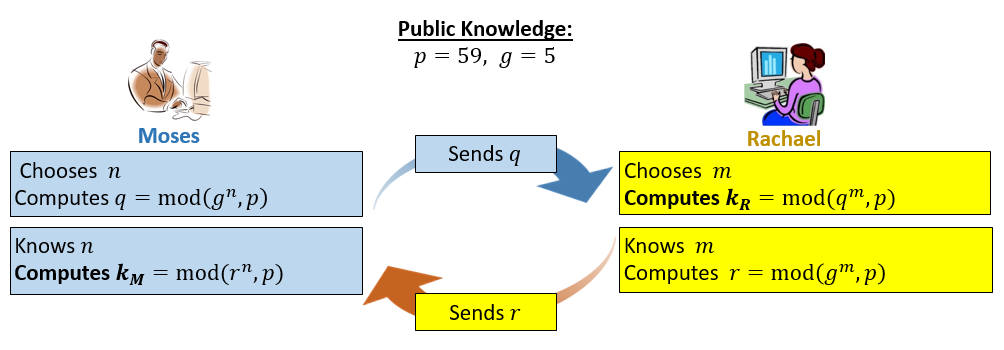
\includegraphics[width=5.5in]
	         {images/DHKE_1.png}}
	  \caption{\label{fig:DH:DHKE_1} Key exchange between Moses and Rachael using DHKE}
\end{figure}

\begin{exercise}{k1isk2}\\
Fill in the blanks in the following proof that  $K_1$ is always equal to  $K_2$.\\
  	\begin{proof} 
		\begin{align*} 
		K_1 &=   \bmod (r^n , \underline{~~~~~~}) 
           	\\&=  \bmod ( \underline{~~~~}^{\underline{~~~~~~}} , p) , p )&& \text{(substitution)}	%ans: \bmod ( \bmod (g^m , p)^n , p )&& \text{(substitution)}
		\\&= \bmod ( \bmod ((g^{\underline{~~~~~~}}) , p) , p )&&  \text{(rules of exponents)}	%ans: \bmod ( \bmod ((g^{mn}) , p) , p )&&  \text{(rules of exponents)}	
           	\\&= \bmod ( \bmod ((\underline{~~~~~~})^{\underline{~~~~~~}} , p) , p )  &&\text{(rules of exponents)}	%ans:  \bmod ( \bmod ((g^n)^m , p) , p )  &&\text{(rules of exponents)}
           	\\&= \bmod (\underline{~~~~~~}^m , p )&&\text{(substitution)}   	%ans: \bmod ( \bmod ((g^n , p)^m , p )&&\text{(substitution)}
		\\&= K_2
		\end{align*} 
   	Thus, $K_1 = K_2 = K$ is a symmetric key.\\

  	\end{proof}
\end{exercise}

Now that you understand the process for DHKE, follow the example below.  (Note that this example is just to give you the idea--it's much too simple to use in practical applications.)

 \begin{eg} Key Exchange between a sender and receiver (Moses and Rachael) using the DHKE is shown in the following steps.
\begin{enumerate}[Step 1.]
\item Prior to sending data, Moses and Rachael agree $p$ = 13 and $g$= 7; 
\item Moses chooses $n$ = 2, and sends Rachael $\bmod (7^2 , 13) = 10$;
\item Rachael chooses $m$ = 8, and sends Moses $\bmod (7^8  , 13) = 3 $;
\item Moses computes $\bmod ((3)^2 , 13 ) = 9$;
\item Rachael computes $\bmod ((10)^8 , 13 ) = 9$;
\item Moses and Rachael share the number 9;
\end{enumerate}
\end{eg}

%  \emph{Fermat's Little Theorem}\index{Fermat's Little Theorem! in cryptography} states that if $p$ is a prime number such that $p \nmid a$, and $a$ is an integer, then $1 \equiv \bmod(a^{p-1}, p)$.

%\begin{eg} Let $p = 5$ and $a = 1, 2, 3, 4 \text{ and } 5$
%$$ 5 \nmid 1 \implies \bmod(1^{5-1}, 5) \equiv 1$$
%$$ \bmod(1^{4}, 5) \equiv 1$$
%$$ \bmod(1, 5) \equiv 1$$
%$$ 5 \nmid 2 \implies \bmod(2^{5-1}, 5) \equiv 1$$
%$$ \bmod(2^{4}, 5) \equiv 1$$
%$$ \bmod(16, 5) \equiv 1$$
%$$ 5 \nmid 3 \implies \bmod(3^{5-1}, 5) \equiv 1$$
%$$ \bmod(3^{4}, 5) \equiv 1$$
%$$ \bmod(18	, 5) \equiv 1$$
%$$ 5 \nmid 4 \implies \bmod(4^{5-1}, 5) \equiv 1$$
%$$ \bmod(4^{4}, 5) \equiv 1$$
%$$ \bmod(256, 5) \equiv 1$$
%$$ 5 | 5 \text { (so the theorem does not apply)}$$
%$$ \bmod(5^{5-1}, 5) \equiv 0$$

%Since all values of $a$ such that $1 \leq a \leq p$ are congruent to $1$, then Fermat's Little Theorem tells us that $p$ is prime, but are there numbers that exist that pass Fermat's Little Theorem but are not prime?  The answer is yes, these numbers are called \emph{Lucas-Carmichael Numbers}\index{Lucas-Carmichael Numbers! in cryptogaphy}.  (or \emph{pseudoprimes}\index{Pseudoprimes}) 

Following the example above you can see that the DHKE requires that you raise a given number $g$ to a natural number (either $m$ or $n$) and take the result mod $p$. This operation is called \term{discrete exponentiation}. Calculating discrete exponentials with small values of $m$ or $n$ is manageable, but in practice the exponent $m$ or $n$ can be enormous, with hundreds of digits. It would seem that in this case discrete exponentiation would take a long, long time to compute.  But we can use the repeated squaring formula described in Section \ref{exercise:crypt:power} to speed up the process.  

You may create a spreadsheet using the repeated squaring formula (or use \url{www.wolframalpha.com}) to find answers to the following exercises.
 
\begin{exer}
Given $p$ = 32452867; $g$ = 54321; and $n$ = 876.  
\begin{enumerate}[(a)]
\item What number do you send?  
%ans: mod((54321)876, 32,452,867) = 19,439,625

\item Alice sends back 31975948.  What is your shared key with Alice? 
%ans: K = mod((31,975,948)876, 32,452,867) = 16,045,878

\item  Bob receives your number from (a) and chooses $m$ = 127. What number does he send back to you? And what is your shared key with Bob?
%ans: K = mod((19,439,625)124, 32,452,867) = 22721372

\item
By an amazingly lucky chance, Alice's choice of $m$ just happens to be very close to Bob's choice.  What is Alice's choice of $m$?
\end{enumerate}
\end{exer}

\begin{exer}
Given $p$ = 86028157; $g$ = 98765; and $n$ = 123.  
\begin{enumerate}[(a)]
\item	What number do you send?  
%ans: mod((98765)123, 86,028,157) = 7,262,961

\item Carol sends back 53161396. What is your shared key? 
%ans: K = mod((53,161,396)123, 86,028,157) = 35,164,864

\item Deborah receives your number from (a) and chooses $m$ = 81. what number does she send to you? And what is your shared key with Deborah?
% K = 5998268

\item
By an extraordinarily lucky chance, Deborah's choice of $m$ just happens to be not too far from Carol's choice.  What is Carol's choice of $m$?
% 87

%ans: K = mod((7,262,961)87, 86,028,157) = 35,164,864
\end{enumerate}
\end{exer}
Now that we understand the DHKE process, let's try to understand why it effectively guarantees the secrecy of the shared key. First, we need to understand a little more about the operation of discrete exponentiation, which (as we've seen) is the foundation of the DHKE process. So we're going on a short digression, but don't worry--we'll get back to the main point shortly. 

In previous math courses you learned that the inverse operation of exponentiation is taking the logarithm: for example, $2^3 = 8$ while $\log_{2}8 = 3$.  It's possible to do the same with discrete exponentiation: the inverse operation to discrete exponentiation is  called \term{discrete logarithm} or (DL). Note that since discrete exponentiation involves raising to a power which is a natural number, the DL will always be a natural number.   For example, since $\bmod(2^5,7)=4$, we could say that under multiplication mod 7,  $5$ is a DL  of $4$ with base $2$. Now why did we say, ``\emph{a} DL'' rather than ``\emph{the} DL''? Because  there happens to be more than one:

\begin{exercise}{DLex1}
\begin{enumerate}[(a)]
\item
Find all natural numbers $n$ such that $\bmod(2^n,7)=4$.  Use your result to complete the following sentence: ``Under multiplication mod 7, the discrete logarithm(s) of $4$ with base 2  are \ldots.''
\item
Find all natural numbers $n$ such that $\bmod(2^n,7)=3$.  Use your result to complete the following sentence:  ``Under multiplication mod 7, the discrete logarithm(s) of $3$ with base 2 are \ldots.''
\item
Find all nonzero elements of $\mathbb{Z}_7 \setminus \{0\}$ which have no discrete logarithms with base 2.
\item
Find all nonzero elements of $\mathbb{Z}_7 \setminus \{0\}$ which have no discrete logarithms with base 3.
\end{enumerate}
\end{exercise}

The preceding exercise points out some key issues with discrete logarithms. Sometimes there are lots of them, and sometimes there aren't any! These phenomena are related to the one-to-oneness and ontoness properties of  the discrete exponential function (recall Definitions~\ref{121defn} and \ref{ontoDef}, respectively):

\begin{exercise}{DLex2}
\begin{enumerate}[(a)]
\item
We may define a function $f: \mathbb{N} \rightarrow \mathbb{Z}_7 \setminus \{0\}$ by the equation: $f(n) = \bmod(2^n,7)$. 
Use parts (a) and (b) of Exercise~\ref{exercise:Crypto:DLex1} to prove that $f$ is neither one-to-one nor onto.
\item
We may also define a function $g: \mathbb{N} \rightarrow \mathbb{Z}_7 \setminus \{0\}$ by the equation: $f(n) = \bmod(3^n,7)$. 
Prove or disprove: $g$ is one-to-one.
\item
With the same $g$ as in part (b), prove or disprove: $g$ is onto.
\end{enumerate}
\end{exercise}

This exercise suggests the following question:  Under what conditions can we guarantee that the discrete exponentiation function is onto and/or one-to-one? (This turns out to be more than an idle question, as we shall see shortly.)  To gain some leverage against this problem, we'll make use of   Proposition~\ref{proposition:poly:Up_cyclic} from Chapter~\ref{poly}, which tells us that the multiplicative group $\mathbb{Z}_p\setminus \{0\}$ is \emph{cyclic}, whenever $p$ is a prime. (In Chapter~\ref{poly} we also used the notation $U(p)$ instead of $\mathbb{Z}_p\setminus \{0\}$, and we'll use this same notation in the following.) This means that for any prime $p$, there is a $g \in U(p)$  such that $g$ is a \emph{generator}\footnote{A generator of $U(p)$ is also referred to as a \term{primitive element} of $\mathbb{Z}_p$.} of  $U(p)$: that is, $U(p) = \langle g \rangle$ (recall from Chapter~\ref{groups} that for a finite group, $\langle g \rangle = \{g, g^2, g^3, \ldots \}$). 
Thus any element of $U(p)$ may be expressed as a power of $g$ (under mod $p$ multiplication).  In other words, the discrete exponentiation function $f: \mathbb{N} \rightarrow U(p)$ given by $f(n) = \bmod(g^n,p)$ is an onto function!  

It turns out that onto-ness also gives use one-to-oneness, when we restrict $f$ to the appropriate domain:

\begin{exercise}{} 
\begin{enumerate}[(a)]
\item
Define $h: U(13) \rightarrow U(13)$ by: $h(n) = \bmod(2^n,13)$.  (Note that the domain of $h$ is restricted to $U(13)$.)  Show that $h$ is a bijection.
\item
Find another number $k \in U(13)$ such that $h: U(13) \rightarrow U(13)$ given by $h(n) = \bmod(k^n,13)$ is also a bijection.
\item
Suppose that $p$ is a prime, and $g$ is a generator of $p$.  Consider the function $f: U(p) \rightarrow U(p)$ given by $f(n) = \bmod(g^n,p)$.  (Note that $f$ is the same as the discrete exponentiation function defined above, except the domain has been restricted.)  Show that $f$ is a bijection.
\end{enumerate}
\end{exercise}

It's about time we got back to the main point. Why do we even care about DL anyway? Well, suppose an eavesdropper who's listening in on Moses and Rachael's conversation wants to figure out the secret key. 
The eavesdropper knows $p, g, q=\bmod(g^n,p)$, and $r=\bmod(g^m,p)$.  This is all the information he has in order to figure out the shared key, which is  $K=\bmod(g^{mn},p)$. If he could figure out $m$ he'd be golden, because then he could compute $\bmod(q^m,p)$ which is equal to $K$. But this is none other than a DL problem, since $m$ is a DL of $r$ with base $g$ under multiplication mod $p$.  

There's an issue that we should address here. We've pointed out that any DL problem has many different solutions. What if the eavesdropper finds a different solution to the DL problem, which is not equal to the $m$ originally used by Rachael? It turns out that the eavesdropper can crack the code with \emph{any} DL solution, as the following exercise shows:

\begin{exercise}{DLex3}
We've just stated that ``$m$ is a DL of $r$ with base $g$ under multiplication mod $p$''.  But we already know there are \emph{many} DL's, not just one. Let $m'$ be a \emph{different} DL of $r$ with base $g$ under multiplication mod $p$. Show that $\bmod(g^{mn},p)=\bmod(g^{m'n},p)$. In other words, an eavesdropper can use \emph{any} DL of $r$ with base $g$ under multiplication mod $p$ to find the shared key.
\end{exercise}

\begin{exercise}{DLex4}
Suppose another eavesdropper was able to compute a DL of $q$ with base $g$ under multiplication mod $p$.  Explain how she could use this information to find Moses and Rachael's secret shared key.
\end{exercise}

The security of the DHKE leverages the easy computation of the discrete exponentials versus the difficulty of computing DL's. (A function which is easy to compute but hard to invert is referred to as a \term{one-way function}. Discrete exponentials (for suitable $p$'s and $g$'s) form a very important class of one-way functions.)
The following simple example introduces how this works in practice. 

\begin{example}{one-way}
It is easy to calculate $\bmod(2^{m},  11)$ for different values of $m$: for example, when $m =8$ then we get $\bmod(2^{8},  11) =\bmod(256,  11)  = 3$.  However, when you try to invert the process, you have: given $\bmod(2^{m},  11) = 3$, calculate $m$. There is no easy way to do this. As you can see below the results jump around, and each solution is equally likely to be an integer between 0 and 11. 
$$ \bmod(2^{1}, 11)=2$$
$$ \bmod(2^{2}, 11)=4$$
$$ \bmod(2^{3}, 11)=8$$
$$ \bmod(2^{4}, 11)=5$$
$$ \bmod(2^{5}, 11)=10$$
$$ \bmod(2^{6}, 11)=9$$
$$ \bmod(2^{7}, 11)=7$$
$$ \bmod(2^{8}, 11)=3$$
$$ \bmod(2^{9}, 11)=6$$
$$ \bmod(2^{10}, 11)=1$$
\end{example}
If you try to calculate $m$ using a brute force method (that is, computing all possible solutions one at a time), you would have to calculate 8 different solutions before you find the right answer. 

The larger the modulus, the harder the DL is to find. The exercise below is designed to show how many computations a brute force attack would take in comparison to a growing modulus.

\begin{exercise}{DLP}
Use the Repeated Square spreadsheet from Exercise \ref{exercise:crypt:power} to solve the following DL Problems. In each case, write down how many discrete exponentials you need to compute in order to find the answer.  
\begin{enumerate}[(a)]
\item Given $ \bmod(7^{m}, 41)=28$, solve for $m$.
%ans: 29

\item Given $ \bmod(5^{m}, 73)=13$, solve for $m$.
%ans: 59

\item Given $ \bmod(17^{m}, 211)=161$, solve for $m$.
%ans: 161

\item
What trend do you see in the number of computations required in parts (a), (b), (c), and how does it relate to the moduli in the different cases?
\end{enumerate}
\end{exercise}

\subsection{Man in the middle attack}
Our previous discussion indicates the DHKE is very hard to crack if it uses a large enough modulus $p$ and a suitable base $g$. But, is there any way to successfully eavesdrop on Moses and Rachael's conversation without actually cracking the code?  Both Moses and Rachael seem confident with the security the DHKE provides, since an attacker would only be privy to $\bmod (g^n , p)$ and $\bmod (g^m , p)$, each of which cannot be used to decrypt the message since an attacker would have to compute the DL problem to find $m$ and $n$. 

But, what would happen if an attacker, Fred (an eavesdropper) places himself between Moses and Rachael's messages?  If Fred could do this then Rachael's message would pass through Fred first before reaching Moses, and vice-versa. Now, Fred can intercept the public key and can establish his own private key with Moses and Rachael.  Fred is now able to read or alter messages.  This type of attack is commonly referred to as the Man in the Middle (MiM) attack.  See Figure~\ref{fig:DH:DHKE_2} to see how Fred is able to modify the Key Exchange.
\begin{figure}[H]
	   \center{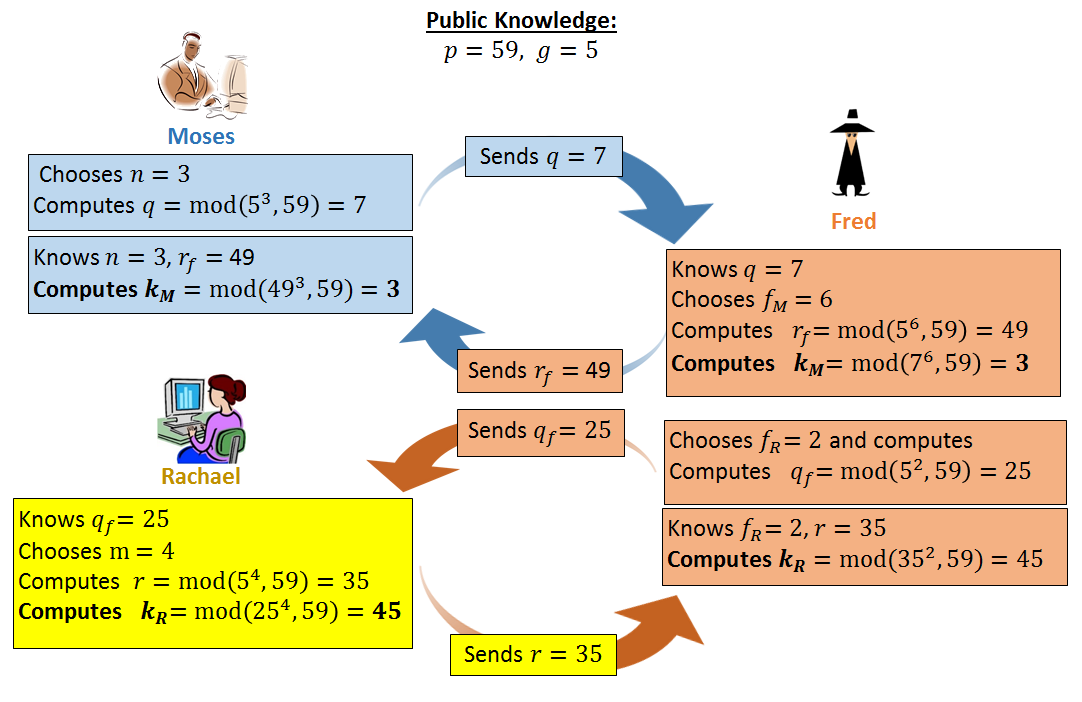
\includegraphics[width=5in]
	         {images/DHKE_18.png}}
	  \caption{\label{fig:DH:DHKE_2} MiM Attack during Moses and Rachael's Key Exchange }
\end{figure}

Following Figure~\ref{fig:DH:DHKE_2}, Fred establishes a secret key $k_M$ with Moses and another secret key $k_R$ with Rachael.  Now Moses thinks he has Rachael's public key, and Rachael thinks that she has Moses' public key. Moses and Rachael both combine their private keys with Fred's public keys and create two different symmetric keys, $K_M$ and $K_R$ respectively. At this point if Moses or Rachael sends a message then Fred is free to decrypt and encrypt the message using the appropriate symmetric key. 

DHKE is vulnerable to this type of MiM attack since Moses cannot verify that Rachael was the originator of the message, and vice-versa.  Preventing a MiM is difficult, but you can overcome a MiM attack using a \term{digital signature}, a digital signature is an electronic signature that encrypts data.  This digital signature serves two purposes: first, it authenticates the origin of the sender and second, it ensures the integrity of the message.  Generally in RSA, a public key is used to encrypt and a private key is used to decrypt (see Section \ref{sec:RSA}.  However, the reverse is more secure.  A message is encrypted using the private key and is decrypted using a public key (asymmetric cryptography). Although digital signatures cannot prevent eavesdropping, they can ensure that false messages are not authenticated. In the next section, we'ill examine the second of these alternatives. 

\section{Elliptic Curve Cryptography}\label{sec:ECC:2}

Elliptic Curve Cryptography (ECC) is one approach to the public key sharing dilemma that offers a smaller security level-to-key lenth ratio (see table below for the relationship  of security and key lengths).  In a cryptosystem the key length is the number of bits in the key (in DHKE the size of the symmetric key is $K1$).  For comparison a 160 bit key has 49 decimal digits, while a 1024 bit key has 309 decimal digits. 

The strength of a cryptography security level is also measured in bits (80, 128, 192, 256, etc.), and each security bit represents the number of computational steps necessary to find a solution.  For example, a security level of 80 means that $2^{80}$ computations are required to break the code. Referencing the table below, we can see that ECC with a 160 bit Finite Field has a similar security level to RSA and Diffie Hellman with 1024-bit moduli. To give you an idea of security level strength, "in 2002 it took $10^4$ computers (mainly PCs) running 24 hours a day for 549 days" to solve an EC with a 109 bit key length. 
\begin{figure} [H]
	   \center{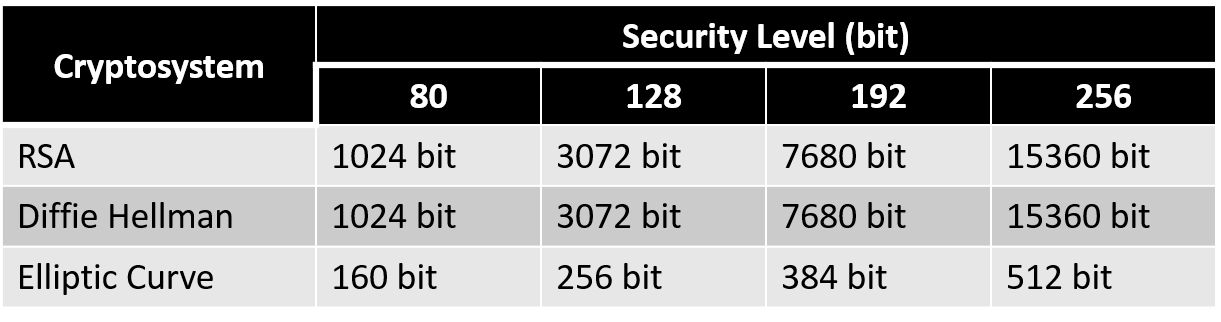
\includegraphics[width=5in]
	         {images/DHKE_9.png}}
	  \caption{\label{fig:DH:DHKE_9} Key bit lengths of Cryptosystems for different security levels recommended by the National Institute of Standards and Technology, retrieved from 
\url{http://resources.infosecinstitute.com/ecc-case-mobile-encryption/}}
\end{figure}
Now that we have established that elliptic curves provide more security with a smaller key size, lets examine the type of elliptic curves we need to use.

\subsection{Elliptic Curves}
An elliptic curve is an algebraic curve defined by the equation, $y^2 = x^3 + ax + b$.  See Figure~\ref{fig:DH:DHKE_5} below for different geometrical representations of elliptic  curves.  
\begin{figure}[H]
	   \center{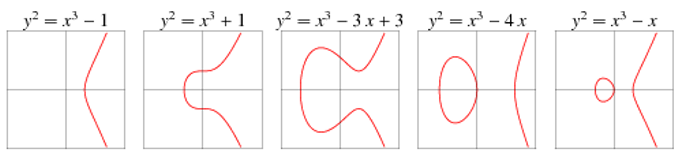
\includegraphics[width=5in]
	         {images/DHKE_5.png}}
	  \caption{\label{fig:DH:DHKE_5}  Geometric shapes of elliptic curves }
\end{figure}
Additionally, the Elliptic Curve (EC) is not allowed to have a double or triple root.  A triple root produces a singularity in the graph, and a double root produces a self-intersection (see graphs in Figure~\ref{fig:DH:DHKE_10}).  It turns out that we can guarantee that the EC has no double or triple roots if the coefficients $a$ and $b$ satisfy the following equation: $4a^3 + 27b^2 \neq 0$.  See graphs in Figure~\ref{fig:DH:DHKE_10} for a geometrical representation.
\begin{figure}[H]
	   \center{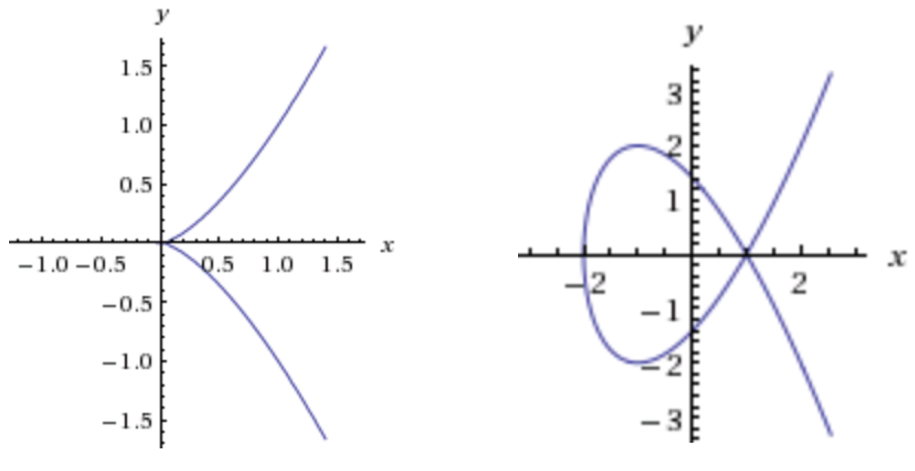
\includegraphics[width=3in]
	         {images/DHKE_10.png}}
	  \caption{\label{fig:DH:DHKE_10} E: $ y^2$ = $x^3$ and E: $ y^2$ = $x^3+ax+b$ }
\end{figure}
\begin{exercise}{}
		\begin{enumerate}[(a)] 
	\item  Prove that if the equation $y^2 = x^3 + ax + b$ has a double root or triple root, then $4a^3+27b^2=0$. (Hint:  if there's a double root , then it must be the case that $0 = x^3 + ax + b$ has a double root. This means that the equation can be factored:  $x^3 + ax+b = (x-r_1)^2(x-r_2)$.  See if you can express $r_1$ and $r_2$ in terms of $a$ and $b$.)\\
	\item Show that if $4a^3 + 27b ^2=0$, then the equation has a double root.  (Hint: there are 2 cases: (i) $b=0$, (ii) $b \neq 0$. In the case $b \neq 0$, first, show that $a > 0$.  Then use part (a) to express $r_1$ and $r_2$ in terms of $a$ and $b$, and show the equation factors properly.
\end {enumerate} 
\end{exercise}

Elliptic curves with coefficients in $\mathbb{R}$ are not used in practical applications, because it is impossible for computers to compute decimal fractions exactly.  The next section will discuss the elliptic curve group.

\subsection{Elliptic Curve Groups}
Given the right type of EC we can use the shape of the EC to conduct specific mathematical operations. A group operation, within the parameters of the EC, is sometimes referred to as addition and is given by two points on the EC, $P_1$, $P_2$ $\in$ E then $P_1 + P_2$ = $P_3$ .  The elements of the group are the points on the elliptic curve.  See below for the EC Group Properties.

\begin{enumerate}[1.]
\item \textbf{Identity}: There is no point on the curve that can serve as a neutral or identity element.  So we artificially define a point at infinity, to serve as the identity element, and it will be directly vertical of the point. 
\begin{figure}[H]
	   \center{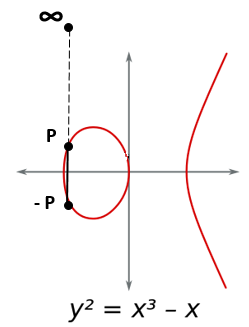
\includegraphics[width=2.5in]
	         {images/DHKE_13.png}}
	  \caption{\label{fig:DH:DHKE_13} Identity property for EC}
\end{figure}
\item \textbf{Inverse}: If you draw a line connecting $\infty$ with $P_1$ the intersection is $-P_1$. So, given a point $P$, the inverse is the point symmetric about the x-axis. 
\begin{figure}[H]
	   \center{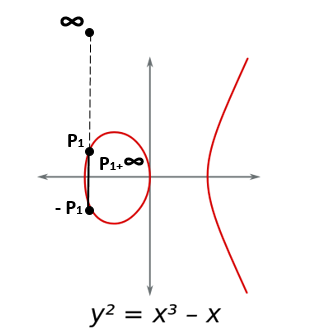
\includegraphics[width=2.5in]
	         {images/DHKE_14.png}}
	  \caption{\label{fig:DH:DHKE_14} Inverse property for EC }
\end{figure}
\item \textbf{closure}: if $P_1$ and $P_2$ are points on the elliptic curve the $P_1 + P_2$ is also a point on the curve;
\item \textbf{associativity}:$(P_1 + P_2) + P_3 = P_1 + (P_2 + P_3)$;
\begin{figure}[H]
	   \center{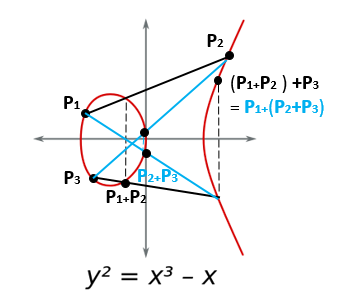
\includegraphics[width=4in]
	         {images/DHKE_12.png}}
	  \caption{\label{fig:DH:DHKE_12} Associative property for EC}
\end{figure}
\end{enumerate}

\begin{eg} Given E: $y^2 = x^3 + 2x + 2 (\bmod17)$, $P_1 = (5,1)$, $P_2 = (5,1)$, and $P_3 = (x_3, y_3)$
	Find $P_3$, where $P_3 = P_1 + P_2$
		\begin{align*}
		\textrm{(1) The slope~} m
		 &= ( (3 \cdot 5^2) + 2) \cdot (2 \cdot 1)^{-1} \bmod 17\\
	          &= (77) \cdot (2)^{-1} \bmod 17\\
                     &\equiv (9) \cdot (9) \bmod 17\\
                     &\equiv 81 \bmod 17\\
                    &\equiv 13
		\end{align*}
		\begin{align*}
		\textrm{(2)~}x_3
		 &= ( (13^2 - 5 - 5  (\bmod 17)) \text{\qquad \qquad \qquad \quad \: \: }\\
	          &= 159(\bmod 17)\\
                     &\equiv 6
		\end{align*}
			\begin{align*}
		\textrm{(3)~}y_3
		 &= ( (13(5 - 6) - 1(\bmod 17)) \text{\qquad \qquad \qquad \quad }\\
	          &= -14(\bmod 17)\\
                     &\equiv 3
		\end{align*}
Thus, $P_3 = (6,3) = 2P$
\end{eg}
\begin {exer}
Using Example 10, find the following: $3P, 4P, 5P, ..., 20P.$  Recall: $3P = 2P + P;  4P = 3P +P;$ etc.  What do you notice about $18P,  19P,$ and $20P?$
\end{exer}
Using Example 10 and Exercise 11, let us reconstruct the Diffie Hellman Key Exchange, but this time we'll use the strength of ECC.  Follow along with Figure~\ref{fig:DH:DHKE_8} below.

\begin{exer}
Using Example 10 and Exercise 11, what is the shared key exchange if Moses chooses $n = 9$ and Rachael chooses $m = 3$?
\end{exer}
\begin{figure}[H]
	   \center{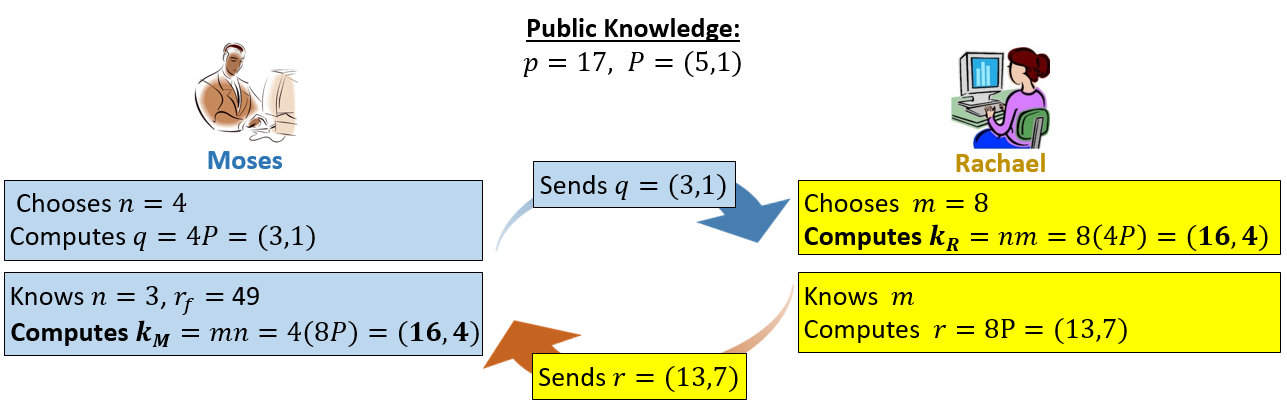
\includegraphics[width=5in]
	         {images/DHKE_8.png}}
	  \caption{\label{fig:DH:DHKE_8} Elliptic Curve Key Exchange between Moses and Rachael }
\end{figure}


\subsection{Elliptic Curve Math}
The elliptic curve protocol is how we perform calculations on the elliptic curve group. First, you must begin from a known point on the elliptic curve called the $generator$.  This point generates the next point which generates the point after that, and the point after that, and so on.  When performing EC math their are two scenarios.  The first is point 1 and point 2 are the same, $P1 = P2$, we'ill talk about how to do this computation a little later on. The second is $P1 \neq P2$. Geometrically if the two points are different then $P_1 + P_2$ is given by drawing a line from point $P_1$ to point $P_2$ and continue the line until it intersects the elliptic curve then reflecting that point about the $x$-axis.  See figure Figure~\ref{fig:DH:DHKE_6} below for a geometric representation.

\begin{figure}[H]
	   \center{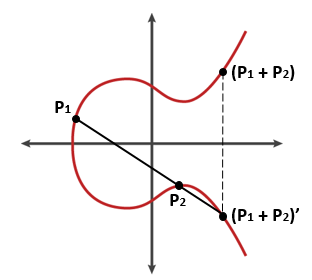
\includegraphics[width=2.5in]
	         {images/DHKE_6.png}}
	  \caption{\label{fig:DH:DHKE_6} Adding  two distinct points, $P_1 + P_2$ on the EC}
\end{figure}

When using Elliptic Curve Cryptography (ECC), the public key is the point on the elliptic curve, and the private key is the number of iterations or "hops" the generator must make to arrive at the public key point.  

It is important to note that $P_1 + P_2$ is always defined on the EC, even though sometimes it may not be apparent.  For instance, take E: $ y^2$ = $x^3 - x$, and points $P_1 = (2, \sqrt{6})$ and $P_2 = (3, \sqrt{24})$.  Then $P_1 + P_2 = (53.65,-377.18)$. See figure Figure~\ref{fig:DH:DHKE_16} below for a graphical representation.
\begin{figure}[H]
	   \center{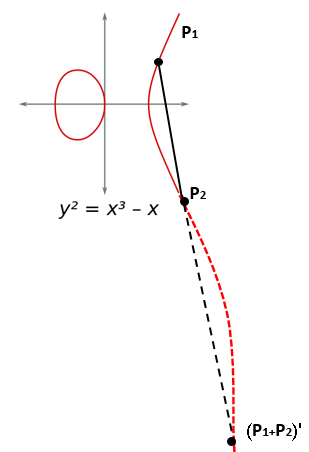
\includegraphics[width=2in]
	         {images/DHKE_16.png}}
	  \caption{\label{fig:DH:DHKE_16} $P_1 + P_2$ is always defined on the EC}
\end{figure}
Given E: $y^2 = x^3 + ax + b$, $P_1 = (x_1, y_1)$, $P_2 = (x_2, y_2)$, and $P_3 = (x_3, y_3)$. Find $P_3$, where $ P_3 =  P_1 + P_2$
\begin{enumerate}[(1)] 
	\item The slope $m =(y_2 - y_1)$ $\cdot$ $(x_2- x_1)^{-1}$, for $P_1$ $\neq$ $P_2$ \\
			\text{ \qquad \: \: \:}or $m = (3x_1^2 + a)$ $\cdot$ $(2y_1)^{-1}$, for $P_1 = P_2$ (this is found by finding\\
			\text{ \qquad \: \: \:}the first derivative of $f(x)$ and plugging the $x$ value into $f'(x)$ \\
			\text{ \qquad \: \: \:}to find the slope at the point)\\
	\item Plug values of $x_2$, $y_2$, and $m$ back into $m =(y_2 - y_1)$ $\cdot$ $(x_2- x_1)^{-1}$ in order to find equation of the line that passes through the two points \\
	\item Use the equation of the line and the equation of the EC to solve for ($x_3, y_3$)
\end {enumerate} 

\begin{eg} Given E: $y^2 = x^3 - 2x$, $P_1 = (0,0)$, $P_2 = (-1,1)$
	Find the line that passes through $P_1 + P_2$
		\begin{enumerate}[(1)] 
	\item The slope $m =(1 - 0)$ $\cdot$ $(-1- 0)^{-1}$ \\
		\text{ \qquad \: \: \:} =$(1)$ $\cdot$ $(-1)^{-1}$ \\
		\text{ \qquad \: \: \:} =-1 
	\item The line through $P_1 + P_2$ \\
		\text{ \qquad \: \:} recall: $y^2 = x^3 - 2x$ \\
		\text{ \qquad \: \:} $y - 1$ = $-1(x- 0)$ \\
		\text{ \qquad \: \:} $y$ =$-x + 1$ 
\end {enumerate} 
\end{eg}

\begin{eg} Given E: $y^2 = x^3 - x$, $P_1 = (2, \sqrt{6})$, $P_2 = (3, \sqrt{24})$ from figure Figure~\ref{fig:DH:DHKE_16} above.
	Find $P_3$, where $P_3 = P_1 + P_2$
		\begin{enumerate}[(1)] 
	\item The slope $m =(\sqrt{6} - \sqrt{24})$ $\cdot$ $(2- 3)^{-1}$ \\
		\text{ \qquad \: \:} or $m = -3\sqrt{6}$ 
	\item $y + \sqrt{24} = -3\sqrt{6}(x - 3)$ \\
		$y = -3\sqrt{6}x + 7\sqrt{6}$
	\item $0 = (-3\sqrt{6}x + 7\sqrt{6})^2 + x^3 - x$\\
		$x \approx 53.65, y \approx -377.18$\\
		$P_3 \approx (53.65, -377.18)$
\end {enumerate}  
\end{eg}

If the two points are the same, $P_1 = P_2$, then a tangent line to the point is drawn and the point of intersection to the EC is then reflected about the x-axis.  This is often referred to as point doubling. See Figure~\ref{fig:DH:DHKE_7} below for a geometrical representation.
\begin{figure}[H]
	   \center{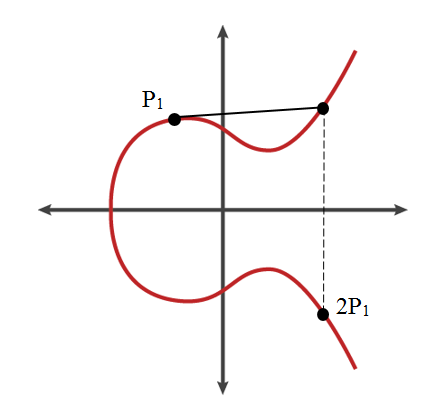
\includegraphics[width=2.5in]
	         {images/DHKE_7.png}}
	  \caption{\label{fig:DH:DHKE_7} Point doubling, adding one point to itself on the EC}
\end{figure}
\subsection{Galois Field} 
As a review, there are three types of algebraic structures: groups, rings, and fields (see Figure~\ref{fig:DH:DHKE_3}); each structure building from the previous structure.  Each structure is defined as a set of elements where: the given operation is closed, has the identity element, has the inverse element, and is associative. For the purpose of this text we'ill focus on Finite Fields (FF), which is a field that contains a finite number of elements and is also known as Galois Fields (GF). Applications of Galois Fields can be seen in CD players, DVD players, disk storage systems, and apps found on computers, tablets and smart phones.
\begin{figure}[H]
	   \center{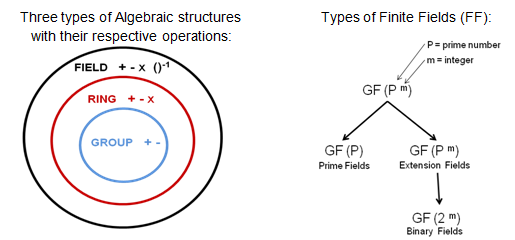
\includegraphics[width=4.5in]
	         {images/DHKE_3.png}}
	  \caption{\label{fig:DH:DHKE_3} Algebraic structures and types of FFs }
\end{figure}
 GFs only exist if they have $P^m$ elements, $GF(P^m)$. So, there is a GF with 27 elements $GF(27) = GF(3^3)$, there is a $GF$ with 256 elements $GF(256) = GF(2^8)$, etc.  In EC we are interested in Binary Fields (BFs), GFs of order $2^m$, with $m ≥ 1$.  Operations in the BF are defined in terms of an irreducible polynomial with degree $m$, this polynomial is also referred to as the reduction polynomial.  This means that the binary polynomial cannot be factored as a product of binary polynomials of degree less than $m$.  There are always $2^m$ elements in $GF(2^m)$, below is an example of the elements in $GF(2^3)$.  
\newline \newline
\begin{eg} Below are the 8 elements of $GF(2^3)$:
\begin{align*}
0, \quad 1, \quad X, \quad X +1, \quad X^2, \quad X^2+1, \quad X^2 + X, \quad X^2 + X + 1
 \end{align*}
\text{Adding two polynomials in $GF(2^3)$ is as follows:}
\begin{align*}
	f(x) &= X^2 + X\\
	g(x) &= X^2  + 1\\
           f(x) + g(x) &= X  + 1
 \end{align*}
 \text{Notice that the addition of the coefficient $X^2$ and the constant 1 = 0 in GF($2^3$)}
\end{eg}
\begin{rem} Given the polynomials $a,b \in  GF(P) = (0,1,2,...,P-1)$ then 
\begin{align*} 		
		a + b &\equiv c (\bmod P)\\
		a - b &\equiv d (\bmod P)\\
		a \cdot b &\equiv e (\bmod P) \quad \text{ ,the multiplicative group does not include 0}\\
		a^{-1} &\equiv b, \mathrm{~if~} \bmod (ab, P) = 1
\end{align*}
\end{rem}	
\begin{exer} Given $GF(2^4)$, add the following two polynomials:
\begin{align*}
	f(x) &= X^3 + X^2 + X + 1\\
	g(x) &= X^2  + 1
 \end{align*}
\end{exer}

\begin{exer} Given $GF(2^8)$, subtract the following two polynomials, $f(x) - g(x)$:
\begin{align*}	
	f(x) &= X^8 +         X^6 +          X^3 + X^2 + 1\\
	g(x) &=        X^7 + X^6 + X^5 +          X^2
\end{align*}
\end{exer}
\begin{rem}
Notice that the binary field has only two coefficients (0,1) so subtraction and addition are the same.
\end{rem}
\begin{eg}Given $GF(2^4)$ and the reduction polynomial $X + 1$, then adding two polynomials is as follows:
\begin{align*}	
	f(x) &=  X^2 + 1\\
	g(x) &= X^3 + X^2 + X + 1\\
	f(x) + g(x) &= X^3 + X (\bmod X + 1)\\
	&= 2X \text{( see below for explanation)}
\end{align*}
\begin{center}
\begin{tabular}{rrcrcrcr}
        &  $x^2$  &  $-$       &$x$&            \\ \cline{2-8}
 \multicolumn{1}{r|}{$x + 1$}
        &  $x^3$  &  $+$  &    &  $+$  & $ x$  \\
        & $x^3$   &  $+$  &    $x^2$ \\ \cline{2-8}
        &         &       &    $-$     $x^2$  &   $+$ &  $x$\\
        &         &       &    $-$     $x^2$  &  $-$  &   $x$  \\ \cline{4-8}
        &         &       &                    &          &   $2x$    &&
\end{tabular}
\end{center}
\end{eg}
\begin{eg} Given $GF(2^4)$ and the reduction polynomial $X^4 + X + 1$, then multiplying two polynomials is as follows:
\begin{align*}	
	f(x) &=  X^2 + X + 1\\
	g(x) &= X^3 + 1\\
 f(x) \cdot g(x) &= X^5 + X^4 + X^3 + X^2 + X + 1 (\bmod X^4 + X + 1)\\ 
	       &= - X^3 - X \text{ , is the remainder (see below for explanation) }
\end{align*}
\begin{center}
\begin{tabular}{rrcrcrcrcrcr}
        &  $x$  &  $+$  &      $1$         \\ \cline{2-12}
 \multicolumn{1}{r|}{$x^4 + x + 1$}
        &  $x^5$  &  $+$  &  $x^4$  &  $+$  & $ x^3$  &  $+$  &  $x^2$  &  $+$  & $ x$  &  $+$  &  $1$  \\
        & $x^5$   &  $+$  &       	&          &      	  &          &  $x^2$   & $+$  &  $x$     \\ \cline{2-12}
        &         &       &         $x^4$  & $+$   &  $ x^3$  &   $+$  &             &         &         &          &  $1$  \\
        &         &       &         $x^4$  &  $+$  &             &           &              &         &  $x$   & $+$  &  $1$   \\ \cline{4-12}
        &         &       &                    &          &   $x^3$ &    $-$  &              &         &  $x$    
\end{tabular}
\end{center}
\end{eg}
We proved the following in Exercise~\ref{exercise:modular:71}.

\begin{prop}{BezoutsIdentity}(\emph{Bezout's Identity})~~ let $x$ and $t$ be two-non-zero integers, and let $d$ be their GCD, then there exists integers $p$ and $a$ such that\\
 \hspace*{\parindent} $px + at = d$
\end{prop}

\begin{corollary}
Using Bezout's Identity we can conclude that if $p$ and $a$ are coprime then we have\\
\hspace*{\parindent} $px + at = 1$ \\
reducing $\bmod p$ yields $at = 1 \bmod p$ .  So $t$ is the multiplicative inverse of\\
 $a$ $\bmod n$.
\end{corollary}

\begin{eg} Given $GF(2^8)$ and the reduction polynomial $X^8 + X^4 + X^3 + X +1$, and $a$ = $X^6 + X^4 + X + 1$ then finding the multiplicative inverse of $a$ is as follows:  $a^{-1}$ = $b$, if $a$ $\cdot$ $b$ $(\bmod p)$ = $1$ .  To find $a^{-1}$ use the Extended Euclidian Algorithm.
\\
	$p =  X^8 + X^4 + X^3 + X +1$\\ 
	$a = X^6 + X^4 + X + 1$\\
\\Using the quotients and remainders found below, we can find the multiplicative inverse of $a$ using the following steps \\(new $t$ = old $t - $quotient $\cdot$ $t$):
\begin{enumerate}
\item $t = 0$
\item new $ t = 1$ 
\item new $t = 0 - 1\cdot(x^2 + 1)$
\item  new $t = 1 - (x^4 + x^2)\cdot(x^2 + 1)$
\item new $t = (x^2 + 1) - (x+1)\cdot(x^6 + x^2 + 1)$
\item Stop here and simplify, since the subsequent remainder is 0.
\item new $t = (x^2 + 1) - (x+1)\cdot(x^6 + x^2 + 1)$ = $x^7 + x^6 + x^3 + x$
\end{enumerate}
Thus, $a^{-1}$ = $x^7 + x^6 + x^3 + x$\\
\begin{center}
\begin{tabular}{rrcrcrcrcrcrcr}
        &  $x^2$  &  $+$  &      $1$         \\ \cline{2-14}
 \multicolumn{1}{r|}{$x^6 + x^4 + x + 1$}
        &  $x^8$  &  $+$  &    &      &  $x^4$  &  $+$  & $ x^3$  &  $+$  &   &   & $ x$  &  $+$  &  $1$  \\
        & $x^8$   &  $+$  &    $x^6$      &    $+$         &      &     &  $x^3$  &  $+$  & $x^2$        \\ \cline{2-14}
        &         &              &$x^6$ &$+$ &  $x^4$  & $+$   &              &          & $ x^2$  &   $+$  & $x$   &  $+$  & $1$       \\
        &         &              &$x^6$ &$+$ &  $x^4$  & $+$   &              &          &   &    & $x$   &  $+$  & $1$   \\ \cline{4-14}
        &         &               &          &      &             &           &       &     & $x^2$ 
\end{tabular}
\end{center}

\begin{center}.

\begin{tabular}{rrcrcrcrcrcrcr}
        &  $x^4$  &  $+$  &      $x^2$      \\ \cline{2-8}
 \multicolumn{1}{r|}{$x^2$}
        &  $x^6$  &  $+$  &    $x^4$  &  $+$   & $ x$  &  $+$  &  $ 1$  \\
        & $x^6$     \\ \cline{2-8}
        &              &           &     $x^4$   & $+$  & $x$   &  $+$   & $1$   \\ 
        &              &           &     $x^4$    \\ \cline{4-8}  
        &              &           &                  &          &  $ x$  &  $+$  &  $ 1$  \\
\end{tabular}
\end{center}

\begin{center}
\begin{tabular}{rrcrcrcrcrcr}
        &  $x$  &  $+$  &      $1$      \\ \cline{2-6}
 \multicolumn{1}{r|}{$x + 1$}
        &  $x^2$  \\
        & $x^2$   &  $+$  &    $x$  \\ \cline{2-6}
        &             &          &    $x$   \\
        &             &          &    $x$  & $+$ & $1$ \\ \cline{4-6}
        &             &          &           &        &  $1$
\end{tabular}
\end{center}

\begin{center}
\begin{tabular}{rrcrcrcrcrcr}
        &  $x$  &  $+$  &      $1$      \\ \cline{2-4}
 \multicolumn{1}{r|}{$1$}
        &  $x$      &   $+$ &    $1$  \\
        & $x$     \\ \cline{2-4}
        &             &          &    $1$   \\
        &             &          &    $1$ \\ \cline{3-4}
        &             &          &    $0$
\end{tabular}
\end{center}

\end{eg}

\begin{exer}
What are the binary elements of GF($2^4$)?
\end{exer}
\begin{exer}
Given GF($2^{12}$), then adding $f(X)$+ $g(X)$ = ?
        \\ $f(X)$ = $X^{10} + X^8 + X^5 + X + 1$
        \\ $g(X)$ = $X^{10} + 1$
\end{exer}
\begin{exer}
Given GF($2^4$), then adding $f(X)$ + $g(X)$ = ?
        \\ $f(X)$ = $X^{2} + X $
        \\ $g(X)$ = $X^{3} + 1$
\end{exer}
\begin{exer}
Given GF($2^5$), then subtracting $f(X)$ + $g(X)$ = ?
        \\ $f(X)$ = $X^{4} + X^2 + 1 $
        \\ $g(X)$ = $X^{3} + 1$
\end{exer}
\begin{exer}
Given GF($2^7$), then subtracting $f(X)$ + $g(X)$ = ?
        \\ $f(X)$ = $X^{6} + X^4 + X $
        \\ $g(X)$ = $X^{3} + 1$
\end{exer}
\begin{exer}
Given GF($2^5$) and the reduction polynomial $X^5 + X + 1$ , then multiplying two polynomials, $f(X)$ $\cdot$ $g(X)$ = ?
        \\ $f(X)$ = $X^{3} + X + 1 $
        \\ $g(X)$ = $X^{4} + X$
\end{exer}
\begin{exer}
Given GF($2^5$) and the reduction polynomial $X^5 + X + 1$ , then multiplying two polynomials, $f(X)$ $\cdot$ $g(X)$ = ?
        \\ $f(X)$ = $X^{4} + X^3 + 1 $
        \\ $g(X)$ = $X^{4} + X^2 + X + 1$
\end{exer}
\begin{exer}
Given GF($2^{160}$) and the reduction polynomial $X^{160} + X + 1$ , then multiplying two polynomials, $f(X)$ $\cdot$ $g(X)$ = ?
        \\ $f(X)$ = $X^{120} + X^{100} + 1 $
        \\ $g(X)$ = $X^{80} + X^{70} + X^{60}$
\end{exer}

\subsection{Elliptic Curve Integrated Encryption System} 
If Moses and Rachael would like to communicate a message using ECC, then they could use an agreed-upon code table and elliptic curve.  Each character of the encrypted message would correspond to a point on the elliptic curve $E_p(a,b)$ where $p$ is a prime number, and Rachael and Moses will have to choose a random point $C$ and $B$ respectively on the EC. Additionally, Rachael selects a random number $\alpha$ which is less than the order of $E_p(a,b)$ and a point $A$ on the EC. She computes $A_1 = $$\alpha$ $(C + A)$ and $A_2= $$\alpha$$A$. Rachael's private keys are $\alpha$ and the point $A$; her public keys are $A_1$ and $A_2$. Moses does the same thing but using $\beta$ and a point $B$. Rachael's public key for Moses is $A_B = $$\alpha$$B_2$, and Moses' public key for Rachael is $B_A = $$\beta$$A_2$. Now lets consider an elliptic curve whose equation is $y^2 = x^3 + 2x + 9$ to see how this works, see Figure~\ref{fig:DH:DHKE_11} below.

\begin{figure}[H]
	   \center{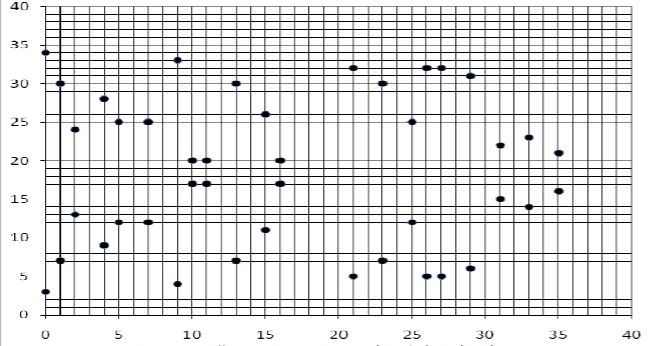
\includegraphics[width=1.5in]
	         {images/DHKE_11.png}}
	  \caption{\label{fig:DH:DHKE_11} Elliptic Curve, $y^2 = x^3 + 2x + 9$ }
\end{figure}

If we choose $37$ as our prime number $p$ then we'll restrict ourselves to the Finite Field, $FF(37)$, so ($y^2 = x^3 + 2x + 9$)$\bmod37$ and use $E_{37}(2,9)$.  Then the points on the elliptic curve are as followed:
($\infty, (5, 25), (1, 30), (21, 32), (7, 25), (25, 12), (4, 28), (0, 34), (16, 17), (15, 26), (27, 32), \newline(9, 4), (2, 24), (26, 5), (33, 14),(11, 17), (31, 22), (13, 30), (35, 21), (23, 7), (10, 17), (29, 6), \newline(29, 31), (10, 20), (23, 30), (35, 16), (13, 7), (31, 15), (11, 20), (33, 23), (26, 32), (2, 13), (9, 33), \newline(27, 5), (15, 11), (16, 20), (0, 3), (4, 9), (25, 25), (7, 12), (21, 5), (1, 7), (5, 12)$)

We can now assign each point on the EC to a character of our choosing and create a code table that will be known to the sender and receiver. Using the table seen in Figure~\ref{fig:DH:DHKE_17} below, Moses and Rachael can now communicate any message to each other.  

\begin{figure}[H]
	   \center{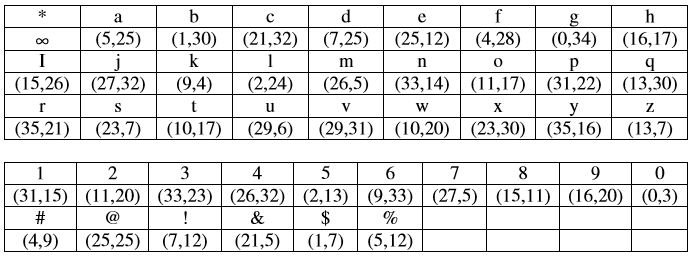
\includegraphics[width=6in]
	         {images/DHKE_17.png}}
	  \caption{\label{fig:DH:DHKE_17} Code table using the EC agreed upon by Moses and Rachael }
\end{figure}

In order for Moses to Encrypt a mesage "M" all of the characters must correspond to points on the EC using the agreed upon table.  The result is a pair of cipher points $(E_1, E_2)$.  Moses chooses a random number, $\gamma$ which changes for each point. So,
$E_1 =$$\gamma$$C$, and $E_2 = M +($$\beta$ $+$$\gamma$$)$$A_1 -$$\gamma$$A_2 + A_B$. After encrypting all characters Moses then converts the pair of points into the text characters using the code table and communicates this message to Rachael.\\

After receiving the cipher text Rachael will decrypt the message using:\\
$M = E_2 - ($$\alpha$ $E_1 +$$\alpha$$B_1 +B_A)$\\

\begin{eg} Moses will send the message, ``attack" using the code table above.\\
First, Rachael and Moses must establish their private and public keys.\\
Rachael lets $C = (9,4)$ and $\alpha$ $= 5$ and $A = (10, 20)$ on the EC. These are her private keys.\\
	$A_1 = 5[(9, 4) + (10, 20)] = (1, 7)$, public key\\
	$A_2 = (32, 23)$, public key\\ \\
Moses lets $B = (11, 20)$ and $\beta$ $= 7$. These are his private keys. \\
	$B_1 = (11, 17)$, public key\\
	$B_2 = (23, 30)$, public key

\begin{flushleft}
Now Moses must encrypt his message one character at a time.
\end{flushleft}
\begin{enumerate}[(1)] 
\item Moses chooses $\gamma$$ = 8$ and encrypts the letter ``a" \newline
	So, the point $(5, 25)$ is encrypted as\newline
	$E_1 = $$\gamma$$C = (1, 30)$ which corresponds to the letter ``b" since $C$ is in the 11th position in the generated table and $\bmod(8 \cdot 11,43) = 2$ and the second position is the character ``b". \newline
	$E_2 = M +($$\beta$ $+$$\gamma$$)$$A_1 -$$\gamma$$A_2 + A_B$ \newline
	$= (5, 25) + 15(1, 7) - 8(32, 23) + (15, 11)$ \newline
	$= 1 + 13 - 17 + 34 = 31\mod 43 = 31 = (2, 13)$ which corresponds to ``5" in the code table.  So, ``a" is encrypted as $(b, 5)$
\item Moses chooses $\gamma$$ = 12$ and encrypts the letter ``t" \newline
	So, the point $(10, 17)$ is encrypted as\newline
	$E_1 = $$\gamma$$C = (21, 32)$ which corresponds to the letter ``c"\newline
	$E_2 = M +($$\beta$ $+$$\gamma$$)$$A_1 -$$\gamma$$A_2 + A_B = (2, 24)$ which corresponds to ``l" in the code table.  So, ``t" is encrypted as $(c, l)$
\item Moses chooses $\gamma$$ = 19$ and encrypts the letter ``t" \newline
	So, the point $(10, 17)$ is encrypted as\newline
	$E_1 = $$\gamma$$C = (4, 9)$ which corresponds to the ``$\#$"\newline
	$E_2 = M +($$\beta$ $+$$\gamma$$)$$A_1 -$$\gamma$$A_2 + A_B = (27, 32)$ which corresponds to ``j" in the code table.  So, ``t" is encrypted as $($$\#$$, j)$
\item Moses chooses $\gamma$$ = 2$ and encrypts the letter ``a" \newline
	So, the point $(5, 25)$ is encrypted as\newline
	$E_1 = $$\gamma$$C = (29, 31)$ which corresponds to the letter ``v"\newline
	$E_2 = M +($$\beta$ $+$$\gamma$$)$$A_1 -$$\gamma$$A_2 + A_B = (1, 30)$ which corresponds to ``b" in the code table.  So, ``a" is encrypted as $(v, b)$
\item Moses chooses $\gamma$$ = 3$ and encrypts the letter ``c" \newline
	So, the point $(5, 25)$ is encrypted as\newline
	$E_1 = $$\gamma$$C = (1, 30)$ which corresponds to the letter ``b"\newline
	$E_2 = M +($$\beta$ $+$$\gamma$$)$$A_1 -$$\gamma$$A_2 + A_B = (31, 22)$ which corresponds to ``p" in the code table.  So, ``c" is encrypted as $(b, p)$
\item Moses chooses $\gamma$$ = 23$ and encrypts the letter ``k" \newline
	So, the point $(9, 4)$ is encrypted as\newline
	$E_1 = $$\gamma$$C = (25, 25)$ which corresponds to ``@"\newline
	$E_2 = M +($$\beta$ $+$$\gamma$$)$$A_1 -$$\gamma$$A_2 + A_B = (4, 28)$ which corresponds to ``f" in the code table.  So, ``a" is encrypted as $(@, f)$
\end{enumerate}
\begin{flushleft}
"attack" is communicated to Rachael as the cypher $(b,5; c,l; $$\#$$,j; v,b; b,p; @,f)$. Rachael is now able to decrypt the cypher text by first converting the characters to their corresponding points, and then uses them to decrypt $M$.
\end{flushleft}
\begin{enumerate}[(1)]
\item $M = E_2 - ($$\alpha$ $E_1 +$$\alpha$$B_1 +B_A) = (5, 25)$ which corresponds to the character ``a" in the code table.\newline
\item $M = E_2 - ($$\alpha$ $E_1 +$$\alpha$$B_1 +B_A) = (10, 17)$ which corresponds to the character ``t" in the code table.\newline
\item $M = E_2 - ($$\alpha$ $E_1 +$$\alpha$$B_1 +B_A) = (10, 17)$ which corresponds to the character ``t" in the code table.\newline
\item $M = E_2 - ($$\alpha$ $E_1 +$$\alpha$$B_1 +B_A) = (5, 25)$ which corresponds to the character ``a" in the code table.\newline
\item $M = E_2 - ($$\alpha$ $E_1 +$$\alpha$$B_1 +B_A) = (21, 32)$ which corresponds to the character ``c" in the code table.\newline
\item $M = E_2 - ($$\alpha$ $E_1 +$$\alpha$$B_1 +B_A) = (9, 4)$ which corresponds to the character ``k" in the code table.\newline
\end{enumerate}
\end{eg} 
It is important to choose a large prime number $p$, in order to make it difficult for an eavesdropper to crack your code.  Computers use a base-2 number system known as the binary number system.  Internet protocols usually use a minimum of a 1024-bit prime number for $p$, which is equivalent to $2^{1024}$ or 300 decimal digits long.  So, there are $2^{1023}$ different possibilities for 1024 bits (where the highest bit is a `1`). It is not necessary to generate your own prime.  There are many records of large primes published that can be referenced. For example, if you visit \url{https://primes.utm.edu/} you can see some lists of 210 digit primes and larger.

\newpage  

\subsection{References and Suggested Reading} 
\begin{enumerate}[(1)]

\item
Azad, Saiful, and Pathan, Al-Sakib Khan. "Elliptic Curve Cryptography" in Practical Cryptography, CRC Press, January 2015.

\item 
Bidgoli, Hossein. "Diffie-Hellman Key Exchange" in \emph{Handbook of Information \newline
Security: Information Warfare, Social, Legal, and International Issues and \newline
Security Foundations, Volume 2}, John Wiley and Sons, January 2006.

\item 
Bos, Joppe, Kaihara, Marcelo, Kleinjung, Thorsten, Lenstra,Arjen,and Montgomery, Peter. (2009, September 01). \emph{On the Security of 1024-bit RSA and 160-bit Elliptic Curve Cryptography}. Retrieved from \url{https://eprint.iacr.org/2009/389.pdf}.

\item 
Christensen, Chris. (2015, November 14). \emph{Key Exchanges}. Retrieved from \url{http://www.nku.edu/~christensen/092mat483}

\item
Franco, Pedro. "Elliptic Curve Cryptography" in \emph{Understanding Bitcoin: Cryptography, Engineering and Economics}, John Wiley and Sons, February 2015.

\item 
Kumar, Suneetha, Chandrasekhar. (2012, January). \emph{Encryption of Data  Using \newline
Elliptic Curve Over Finite Fields}. Retrieved from \newline 
\url{https://arxiv.org/ftp/arxiv/papers/1202/1202.1895.pdf}.

\item 
Mandal, Surajit, Manna, Nilotpal, and Saha, Arijit. "Diffie-Hellman \newline
Key Exchange" in \emph{Information Theory, Coding, and Cryptography}, Pearson India, May 2013.

\item 
Pomerance, Carls. (n.d.). \emph{Discrete Logarithms}. Retrieved from \url{https://math.dartmouth.edu/~carlp/dltalk09.pdf}.




\end{enumerate}
\clearpage
\addcontentsline{toc}{chapter}{Index}
\printindex

%% RAB, 2009/01/28
%% Include GFDL as an appendix
%%
%% To build index with included sectioning info via "style file" execute:
%% makeindex -s aata-index-style.ist aata.idx
%% See:  http://www.troubleshooters.com/linux/lyx/makeindex.htm
%% Needs "\phantomsection", http://www.tug.org/applications/hyperref/manual.html
%
\backmatter
%
%\include{solution}
%{\small%%%%(c)
%%%%(c)  This file is a portion of the source for the textbook
%%%%(c)
%%%%(c)    Abstract Algebra: Theory and Applications
%%%%(c)    Copyright 1997 by Thomas W. Judson
%%%%(c)
%%%%(c)  See the file COPYING.txt for copying conditions
%%%%(c)
%%%%(c)
\chapter*{GNU Free Documentation License}

\addcontentsline{toc}{chapter}{GNU Free Documentation License}
\pagestyle{myheadings}
\markboth{GFDL LICENSE}{GFDL LICENSE}

 \begin{center}

       Version 1.2, November 2002


 Copyright \copyright{} 2000,2001,2002  Free Software Foundation, Inc.
 
 \bigskip
 
     51 Franklin St, Fifth Floor, Boston, MA  02110-1301  USA
  
 \bigskip
 
 Everyone is permitted to copy and distribute verbatim copies
 of this license document, but changing it is not allowed.
\end{center}


\begin{center}
{\bf\large Preamble}
\end{center}

The purpose of this License is to make a manual, textbook, or other
functional and useful document ``free'' in the sense of freedom: to
assure everyone the effective freedom to copy and redistribute it,
with or without modifying it, either commercially or noncommercially.
Secondarily, this License preserves for the author and publisher a way
to get credit for their work, while not being considered responsible
for modifications made by others.

This License is a kind of ``copyleft'', which means that derivative
works of the document must themselves be free in the same sense.  It
complements the GNU General Public License, which is a copyleft
license designed for free software.

We have designed this License in order to use it for manuals for free
software, because free software needs free documentation: a free
program should come with manuals providing the same freedoms that the
software does.  But this License is not limited to software manuals;
it can be used for any textual work, regardless of subject matter or
whether it is published as a printed book.  We recommend this License
principally for works whose purpose is instruction or reference.

\section*{1.\ Applicability And Definitions}
% \begin{center}
% {\Large\bf 1. APPLICABILITY AND DEFINITIONS\par}
% \phantomsection
% \addcontentsline{toc}{section}{1. APPLICABILITY AND DEFINITIONS}
% \end{center}

This License applies to any manual or other work, in any medium, that
contains a notice placed by the copyright holder saying it can be
distributed under the terms of this License.  Such a notice grants a
world-wide, royalty-free license, unlimited in duration, to use that
work under the conditions stated herein.  The ``\textbf{Document}'', below,
refers to any such manual or work.  Any member of the public is a
licensee, and is addressed as ``\textbf{you}''.  You accept the license if you
copy, modify or distribute the work in a way requiring permission
under copyright law.

A ``\textbf{Modified Version}'' of the Document means any work containing the
Document or a portion of it, either copied verbatim, or with
modifications and/or translated into another language.

A ``\textbf{Secondary Section}'' is a named appendix or a front-matter section of
the Document that deals exclusively with the relationship of the
publishers or authors of the Document to the Document's overall subject
(or to related matters) and contains nothing that could fall directly
within that overall subject.  (Thus, if the Document is in part a
textbook of mathematics, a Secondary Section may not explain any
mathematics.)  The relationship could be a matter of historical
connection with the subject or with related matters, or of legal,
commercial, philosophical, ethical or political position regarding
them.

The ``\textbf{Invariant Sections}'' are certain Secondary Sections whose titles
are designated, as being those of Invariant Sections, in the notice
that says that the Document is released under this License.  If a
section does not fit the above definition of Secondary then it is not
allowed to be designated as Invariant.  The Document may contain zero
Invariant Sections.  If the Document does not identify any Invariant
Sections then there are none.

The ``\textbf{Cover Texts}'' are certain short passages of text that are listed,
as Front-Cover Texts or Back-Cover Texts, in the notice that says that
the Document is released under this License.  A Front-Cover Text may
be at most 5 words, and a Back-Cover Text may be at most 25 words.

A ``\textbf{Transparent}'' copy of the Document means a machine-readable copy,
represented in a format whose specification is available to the
general public, that is suitable for revising the document
straightforwardly with generic text editors or (for images composed of
pixels) generic paint programs or (for drawings) some widely available
drawing editor, and that is suitable for input to text formatters or
for automatic translation to a variety of formats suitable for input
to text formatters.  A copy made in an otherwise Transparent file
format whose markup, or absence of markup, has been arranged to thwart
or discourage subsequent modification by readers is not Transparent.
An image format is not Transparent if used for any substantial amount
of text.  A copy that is not ``Transparent'' is called ``\textbf{Opaque}''.

Examples of suitable formats for Transparent copies include plain
ASCII without markup, Texinfo input format, LaTeX input format, SGML
or XML using a publicly available DTD, and standard-conforming simple
HTML, PostScript or PDF designed for human modification.  Examples of
transparent image formats include PNG, XCF and JPG.  Opaque formats
include proprietary formats that can be read and edited only by
proprietary word processors, SGML or XML for which the DTD and/or
processing tools are not generally available, and the
machine-generated HTML, PostScript or PDF produced by some word
processors for output purposes only.

The ``\textbf{Title Page}'' means, for a printed book, the title page itself,
plus such following pages as are needed to hold, legibly, the material
this License requires to appear in the title page.  For works in
formats which do not have any title page as such, ``Title Page'' means
the text near the most prominent appearance of the work's title,
preceding the beginning of the body of the text.

A section ``\textbf{Entitled XYZ}'' means a named subunit of the Document whose
title either is precisely XYZ or contains XYZ in parentheses following
text that translates XYZ in another language.  (Here XYZ stands for a
specific section name mentioned below, such as ``\textbf{Acknowledgements}'',
``\textbf{Dedications}'', ``\textbf{Endorsements}'', or ``\textbf{History}''.)  
To ``\textbf{Preserve the Title}''
of such a section when you modify the Document means that it remains a
section ``Entitled XYZ'' according to this definition.

The Document may include Warranty Disclaimers next to the notice which
states that this License applies to the Document.  These Warranty
Disclaimers are considered to be included by reference in this
License, but only as regards disclaiming warranties: any other
implication that these Warranty Disclaimers may have is void and has
no effect on the meaning of this License.

\section*{2.\ Verbatim Copying}
% \begin{center}
% {\Large\bf 2. VERBATIM COPYING\par}
% %% \phantomsection
% \addcontentsline{toc}{section}{2. VERBATIM COPYING}
% \end{center}

You may copy and distribute the Document in any medium, either
commercially or noncommercially, provided that this License, the
copyright notices, and the license notice saying this License applies
to the Document are reproduced in all copies, and that you add no other
conditions whatsoever to those of this License.  You may not use
technical measures to obstruct or control the reading or further
copying of the copies you make or distribute.  However, you may accept
compensation in exchange for copies.  If you distribute a large enough
number of copies you must also follow the conditions in section~3.

You may also lend copies, under the same conditions stated above, and
you may publicly display copies.

\section*{3.\ Copying In Quantity}
% \begin{center}
% {\Large\bf 3. COPYING IN QUANTITY\par}
% %% \phantomsection
% \addcontentsline{toc}{section}{3. COPYING IN QUANTITY}
% \end{center}


If you publish printed copies (or copies in media that commonly have
printed covers) of the Document, numbering more than 100, and the
Document's license notice requires Cover Texts, you must enclose the
copies in covers that carry, clearly and legibly, all these Cover
Texts: Front-Cover Texts on the front cover, and Back-Cover Texts on
the back cover.  Both covers must also clearly and legibly identify
you as the publisher of these copies.  The front cover must present
the full title with all words of the title equally prominent and
visible.  You may add other material on the covers in addition.
Copying with changes limited to the covers, as long as they preserve
the title of the Document and satisfy these conditions, can be treated
as verbatim copying in other respects.

If the required texts for either cover are too voluminous to fit
legibly, you should put the first ones listed (as many as fit
reasonably) on the actual cover, and continue the rest onto adjacent
pages.

If you publish or distribute Opaque copies of the Document numbering
more than 100, you must either include a machine-readable Transparent
copy along with each Opaque copy, or state in or with each Opaque copy
a computer-network location from which the general network-using
public has access to download using public-standard network protocols
a complete Transparent copy of the Document, free of added material.
If you use the latter option, you must take reasonably prudent steps,
when you begin distribution of Opaque copies in quantity, to ensure
that this Transparent copy will remain thus accessible at the stated
location until at least one year after the last time you distribute an
Opaque copy (directly or through your agents or retailers) of that
edition to the public.

It is requested, but not required, that you contact the authors of the
Document well before redistributing any large number of copies, to give
them a chance to provide you with an updated version of the Document.

\section*{4.\ Modifications}
% \begin{center}
% {\Large\bf 4. MODIFICATIONS\par}
% %% \phantomsection
% \addcontentsline{toc}{section}{4. MODIFICATIONS}
% \end{center}

You may copy and distribute a Modified Version of the Document under
the conditions of sections 2 and 3 above, provided that you release
the Modified Version under precisely this License, with the Modified
Version filling the role of the Document, thus licensing distribution
and modification of the Modified Version to whoever possesses a copy
of it.  In addition, you must do these things in the Modified Version:

\begin{itemize}
\item[A.] 
   Use in the Title Page (and on the covers, if any) a title distinct
   from that of the Document, and from those of previous versions
   (which should, if there were any, be listed in the History section
   of the Document).  You may use the same title as a previous version
   if the original publisher of that version gives permission.
   
\item[B.]
   List on the Title Page, as authors, one or more persons or entities
   responsible for authorship of the modifications in the Modified
   Version, together with at least five of the principal authors of the
   Document (all of its principal authors, if it has fewer than five),
   unless they release you from this requirement.
   
\item[C.]
   State on the Title page the name of the publisher of the
   Modified Version, as the publisher.
   
\item[D.]
   Preserve all the copyright notices of the Document.
   
\item[E.]
   Add an appropriate copyright notice for your modifications
   adjacent to the other copyright notices.
   
\item[F.]
   Include, immediately after the copyright notices, a license notice
   giving the public permission to use the Modified Version under the
   terms of this License, in the form shown in the Addendum below.
   
\item[G.]
   Preserve in that license notice the full lists of Invariant Sections
   and required Cover Texts given in the Document's license notice.
   
\item[H.]
   Include an unaltered copy of this License.
   
\item[I.]
   Preserve the section Entitled ``History'', Preserve its Title, and add
   to it an item stating at least the title, year, new authors, and
   publisher of the Modified Version as given on the Title Page.  If
   there is no section Entitled ``History'' in the Document, create one
   stating the title, year, authors, and publisher of the Document as
   given on its Title Page, then add an item describing the Modified
   Version as stated in the previous sentence.
   
\item[J.]
   Preserve the network location, if any, given in the Document for
   public access to a Transparent copy of the Document, and likewise
   the network locations given in the Document for previous versions
   it was based on.  These may be placed in the ``History'' section.
   You may omit a network location for a work that was published at
   least four years before the Document itself, or if the original
   publisher of the version it refers to gives permission.
   
\item[K.]
   For any section Entitled ``Acknowledgements'' or ``Dedications'',
   Preserve the Title of the section, and preserve in the section all
   the substance and tone of each of the contributor acknowledgements
   and/or dedications given therein.
   
\item[L.]
   Preserve all the Invariant Sections of the Document,
   unaltered in their text and in their titles.  Section numbers
   or the equivalent are not considered part of the section titles.
   
\item[M.]
   Delete any section Entitled ``Endorsements''.  Such a section
   may not be included in the Modified Version.
   
\item[N.]
   Do not retitle any existing section to be Entitled ``Endorsements''
   or to conflict in title with any Invariant Section.
   
\item[O.]
   Preserve any Warranty Disclaimers.
\end{itemize}

If the Modified Version includes new front-matter sections or
appendices that qualify as Secondary Sections and contain no material
copied from the Document, you may at your option designate some or all
of these sections as invariant.  To do this, add their titles to the
list of Invariant Sections in the Modified Version's license notice.
These titles must be distinct from any other section titles.

You may add a section Entitled ``Endorsements'', provided it contains
nothing but endorsements of your Modified Version by various
parties--for example, statements of peer review or that the text has
been approved by an organization as the authoritative definition of a
standard.

You may add a passage of up to five words as a Front-Cover Text, and a
passage of up to 25 words as a Back-Cover Text, to the end of the list
of Cover Texts in the Modified Version.  Only one passage of
Front-Cover Text and one of Back-Cover Text may be added by (or
through arrangements made by) any one entity.  If the Document already
includes a cover text for the same cover, previously added by you or
by arrangement made by the same entity you are acting on behalf of,
you may not add another; but you may replace the old one, on explicit
permission from the previous publisher that added the old one.

The author(s) and publisher(s) of the Document do not by this License
give permission to use their names for publicity for or to assert or
imply endorsement of any Modified Version.

\section*{5.\ Combining Documents}
% \begin{center}
% {\Large\bf 5. COMBINING DOCUMENTS\par}
% %% \phantomsection
% \addcontentsline{toc}{section}{5. COMBINING DOCUMENTS}
% \end{center}


You may combine the Document with other documents released under this
License, under the terms defined in section~4 above for modified
versions, provided that you include in the combination all of the
Invariant Sections of all of the original documents, unmodified, and
list them all as Invariant Sections of your combined work in its
license notice, and that you preserve all their Warranty Disclaimers.

The combined work need only contain one copy of this License, and
multiple identical Invariant Sections may be replaced with a single
copy.  If there are multiple Invariant Sections with the same name but
different contents, make the title of each such section unique by
adding at the end of it, in parentheses, the name of the original
author or publisher of that section if known, or else a unique number.
Make the same adjustment to the section titles in the list of
Invariant Sections in the license notice of the combined work.

In the combination, you must combine any sections Entitled ``History''
in the various original documents, forming one section Entitled
``History''; likewise combine any sections Entitled ``Acknowledgements'',
and any sections Entitled ``Dedications''.  You must delete all sections
Entitled ``Endorsements''.

\section*{6.\ Collections Of Documents}
% \begin{center}
% {\Large\bf 6. COLLECTIONS OF DOCUMENTS\par}
% %% \phantomsection
% \addcontentsline{toc}{section}{6. COLLECTIONS OF DOCUMENTS}
% \end{center}

You may make a collection consisting of the Document and other documents
released under this License, and replace the individual copies of this
License in the various documents with a single copy that is included in
the collection, provided that you follow the rules of this License for
verbatim copying of each of the documents in all other respects.

You may extract a single document from such a collection, and distribute
it individually under this License, provided you insert a copy of this
License into the extracted document, and follow this License in all
other respects regarding verbatim copying of that document.

\section*{7.\ Aggregation With Independent Works}
% \begin{center}
% {\Large\bf 7. AGGREGATION WITH INDEPENDENT WORKS\par}
% %% \phantomsection
% \addcontentsline{toc}{section}{7. AGGREGATION WITH INDEPENDENT WORKS}
% \end{center}


A compilation of the Document or its derivatives with other separate
and independent documents or works, in or on a volume of a storage or
distribution medium, is called an ``aggregate'' if the copyright
resulting from the compilation is not used to limit the legal rights
of the compilation's users beyond what the individual works permit.
When the Document is included in an aggregate, this License does not
apply to the other works in the aggregate which are not themselves
derivative works of the Document.

If the Cover Text requirement of section~3 is applicable to these
copies of the Document, then if the Document is less than one half of
the entire aggregate, the Document's Cover Texts may be placed on
covers that bracket the Document within the aggregate, or the
electronic equivalent of covers if the Document is in electronic form.
Otherwise they must appear on printed covers that bracket the whole
aggregate.

\section*{8.\ Translation}
% \begin{center}
% {\Large\bf 8. TRANSLATION\par}
% %% \phantomsection
% \addcontentsline{toc}{section}{8. TRANSLATION}
% \end{center}


Translation is considered a kind of modification, so you may
distribute translations of the Document under the terms of section~4.
Replacing Invariant Sections with translations requires special
permission from their copyright holders, but you may include
translations of some or all Invariant Sections in addition to the
original versions of these Invariant Sections.  You may include a
translation of this License, and all the license notices in the
Document, and any Warranty Disclaimers, provided that you also include
the original English version of this License and the original versions
of those notices and disclaimers.  In case of a disagreement between
the translation and the original version of this License or a notice
or disclaimer, the original version will prevail.

If a section in the Document is Entitled ``Acknowledgements'',
``Dedications'', or ``History'', the requirement (section~4) to Preserve
its Title (section~1) will typically require changing the actual
title.

\section*{9.\ Termination}
% \begin{center}
% {\Large\bf 9. TERMINATION\par}
% %% \phantomsection
% \addcontentsline{toc}{section}{9. TERMINATION}
% \end{center}


You may not copy, modify, sublicense, or distribute the Document except
as expressly provided for under this License.  Any other attempt to
copy, modify, sublicense or distribute the Document is void, and will
automatically terminate your rights under this License.  However,
parties who have received copies, or rights, from you under this
License will not have their licenses terminated so long as such
parties remain in full compliance.

\section*{10.\ Future Revisions Of This License}
% \begin{center}
% {\Large\bf 10. FUTURE REVISIONS OF THIS LICENSE\par}
% %% \phantomsection
% \addcontentsline{toc}{section}{10. FUTURE REVISIONS OF THIS LICENSE}
% \end{center}


The Free Software Foundation may publish new, revised versions
of the GNU Free Documentation License from time to time.  Such new
versions will be similar in spirit to the present version, but may
differ in detail to address new problems or concerns.  See
http://www.gnu.org/copyleft/.

Each version of the License is given a distinguishing version number.
If the Document specifies that a particular numbered version of this
License ``or any later version'' applies to it, you have the option of
following the terms and conditions either of that specified version or
of any later version that has been published (not as a draft) by the
Free Software Foundation.  If the Document does not specify a version
number of this License, you may choose any version ever published (not
as a draft) by the Free Software Foundation.

\section*{Addendum: How to use this License for your documents}
% \begin{center}
% {\Large\bf ADDENDUM: How to use this License for your documents\par}
% %% \phantomsection
% \addcontentsline{toc}{section}{ADDENDUM: How to use this License for your documents}
% \end{center}

To use this License in a document you have written, include a copy of
the License in the document and put the following copyright and
license notices just after the title page:

\bigskip
\begin{quote}
    Copyright \copyright{}  YEAR  YOUR NAME.
    Permission is granted to copy, distribute and/or modify this document
    under the terms of the GNU Free Documentation License, Version 1.2
    or any later version published by the Free Software Foundation;
    with no Invariant Sections, no Front-Cover Texts, and no Back-Cover Texts.
    A copy of the license is included in the section entitled ``GNU
    Free Documentation License''.
\end{quote}
\bigskip
    
If you have Invariant Sections, Front-Cover Texts and Back-Cover Texts,
replace the ``with \dots\ Texts.'' line with this:

\bigskip
\begin{quote}
    with the Invariant Sections being LIST THEIR TITLES, with the
    Front-Cover Texts being LIST, and with the Back-Cover Texts being LIST.
\end{quote}
\bigskip
    
If you have Invariant Sections without Cover Texts, or some other
combination of the three, merge those two alternatives to suit the
situation.

If your document contains nontrivial examples of program code, we
recommend releasing these examples in parallel under your choice of
free software license, such as the GNU General Public License,
to permit their use in free software.
}
%\include{notation}
%{\small\printindex}
%
%% RAB, 2009/01/28
%% Ditched endnotes for improved notation.tex
%%
%% \include{endnotes}
\end{document}
